\documentclass[format=acmsmall, review=false, screen=false]{acmart}

\usepackage[T1]{fontenc}
\usepackage{booktabs} % For formal tables
\usepackage{amssymb}
\usepackage{amsmath}
%\usepackage[ruled]{algorithm2e} % For algorithms
%\renewcommand{\algorithmcfname}{ALGORITHM}
%\SetAlFnt{\small}
%\SetAlCapFnt{\small}
%\SetAlCapNameFnt{\small}
%\SetAlCapHSkip{0pt}
%\IncMargin{-\parindent}
\usepackage{algorithm}
\usepackage{algpseudocode} % For algorithms
\usepackage{listings} % For listings
\usepackage{subfig} % For subfiges
\usepackage[export]{adjustbox}
\usepackage{caption}
\usepackage{multirow}
\usepackage{array}
\usepackage{enumitem}
\setlist[itemize]{leftmargin=7mm}

\usepackage{amsmath}
% Metadata Information
\acmJournal{TOIT}
\acmVolume{9}
\acmNumber{4}
\acmArticle{39}
\acmYear{2017}
\acmMonth{12}
\copyrightyear{2017}
%\acmArticleSeq{9}

% Copyright
%\setcopyright{acmcopyright}
\setcopyright{acmlicensed}
%\setcopyright{rightsretained}
%\setcopyright{usgov}
%\setcopyright{usgovmixed}
%\setcopyright{cagov}
%\setcopyright{cagovmixed}

% DOI
\acmDOI{0000001.0000001}

% Paper history
\received{December 2017}
\received[revised]{March 2018}
\received[accepted]{June 2009}


% Document starts
\begin{document}
	% Title portion. Note the short title for running heads 
	\title[A Unified Model for the Mobile-Edge-Cloud Continuum]{A Unified Model for the Mobile-Edge-Cloud Continuum}  
	
	%\author{Gang Zhou}
	%\orcid{1234-5678-9012-3456}
	%\affiliation{%
	%  \institution{College of William and Mary}
	%  \streetaddress{104 Jamestown Rd}
	%  \city{Williamsburg}
	%  \state{VA}
	%  \postcode{23185}
	%  \country{USA}}
	%\email{gang_zhou@wm.edu}
	%\author{Valerie B\'eranger}
	%\affiliation{%
	%  \institution{Inria Paris-Rocquencourt}
	%  \city{Rocquencourt}
	%  \country{France}
	%}
	%\email{beranger@inria.fr}
	%\author{Aparna Patel} 
	%\affiliation{%
	% \institution{Rajiv Gandhi University}
	% \streetaddress{Rono-Hills}
	% \city{Doimukh} 
	% \state{Arunachal Pradesh}
	% \country{India}}
	%\email{aprna_patel@rguhs.ac.in}
	%\author{Huifen Chan}
	%\affiliation{%
	%  \institution{Tsinghua University}
	%  \streetaddress{30 Shuangqing Rd}
	%  \city{Haidian Qu} 
	%  \state{Beijing Shi}
	%  \country{China}
	%}
	%\email{chan0345@tsinghua.edu.cn}
	%\author{Ting Yan}
	%\affiliation{%
	%  \institution{Eaton Innovation Center}
	%  \city{Prague}
	%  \country{Czech Republic}}
	%\email{yanting02@gmail.com}
	%\author{Tian He}
	%\affiliation{%
	%  \institution{University of Virginia}
	%  \department{School of Engineering}
	%  \city{Charlottesville}
	%  \state{VA}
	%  \postcode{22903}
	%  \country{USA}
	%}
	%\affiliation{%
	%  \institution{University of Minnesota}
	%  \country{USA}}
	%\email{tinghe@uva.edu}
	%\author{Chengdu Huang}
	%\author{John A. Stankovic}
	%\author{Tarek F. Abdelzaher}
	%\affiliation{%
	%  \institution{University of Virginia}
	%  \department{School of Engineering}
	%  \city{Charlottesville}
	%  \state{VA}
	%  \postcode{22903}
	%  \country{USA}
	%}
	\author{L. Baresi}
	\author{D. F. Mendon\c{c}a}
	\author{M. Garriga}
	\author{S. Guinea}
	\author{G. Quattrocchi}
	\affiliation{%
		\institution{\\Politecnico di Milano}
		\department{Dipartimento di Elettronica, Informazione e Bioingegneria}
		\city{Milan}
		\state{MI}
		\postcode{20133}
		\country{Italy}
	}
	
	
	\begin{abstract}
		Multifrequency media access control has been well understood in
general wireless ad hoc networks, while in wireless sensor networks,
researchers still focus on single frequency solutions. In wireless
sensor networks, each device is typically equipped with a single
radio transceiver and applications adopt much smaller packet sizes
compared to those in general wireless ad hoc networks. Hence, the
multifrequency MAC protocols proposed for general wireless ad hoc
networks are not suitable for wireless sensor network applications,
which we further demonstrate through our simulation experiments. In
this article, we propose MMSN, which takes advantage of
multifrequency availability while, at the same time, takes into
consideration the restrictions of wireless sensor networks. Through
extensive experiments, MMSN exhibits the prominent ability to utilize
parallel transmissions among neighboring nodes. When multiple physical
frequencies are available, it also achieves increased energy
efficiency, demonstrating the ability to work against radio
interference and the tolerance to a wide range of measured time
synchronization errors.\footnote{This is an abstract footnote}
	\end{abstract}
	
	
	%
	% The code below should be generated by the tool at
	% http://dl.acm.org/ccs.cfm
	% Please copy and paste the code instead of the example below. 
	%
	\begin{CCSXML}
		<ccs2012>
		<concept>
		<concept_id>10010520.10010521.10010537.10010538</concept_id>
		<concept_desc>Computer systems organization~Client-server architectures</concept_desc>
		<concept_significance>500</concept_significance>
		</concept>
		<concept>
		<concept_id>10010520.10010521.10010542.10010546</concept_id>
		<concept_desc>Computer systems organization~Heterogeneous (hybrid) systems</concept_desc>
		<concept_significance>500</concept_significance>
		</concept>
		<concept>
		<concept_id>10003456.10003457.10003490.10003503</concept_id>
		<concept_desc>Social and professional topics~Software management</concept_desc>
		<concept_significance>500</concept_significance>
		</concept>
		<concept>
		<concept_id>10010520.10010570.10010574</concept_id>
		<concept_desc>Computer systems organization~Real-time system architecture</concept_desc>
		<concept_significance>500</concept_significance>
		</concept>
		<concept>
		<concept_id>10003120.10003138.10003139.10010905</concept_id>
		<concept_desc>Human-centered computing~Mobile computing</concept_desc>
		<concept_significance>500</concept_significance>
		</concept>
		</ccs2012>
	\end{CCSXML}
	
	\ccsdesc[500]{Computer systems organization~Client-server architectures}
	\ccsdesc[500]{Computer systems organization~Heterogeneous (hybrid) systems}
	\ccsdesc[500]{Computer systems organization~Real-time system architecture}
	\ccsdesc[500]{Social and professional topics~Software management}
	\ccsdesc[500]{Human-centered computing~Mobile computing}
	
	
	%
	% End generated code
	%
	
	
	
	\keywords{computing continuum, edge computing, fog computing, mobile computing, real-time systems, ops automation, functions-as-a-service}
	
	
	
	
	\maketitle
	
	% The default list of authors is too long for headers.
	\renewcommand\shortauthors{Baresi, L. et al}
	\renewcommand{\texttt}[1]{\textit{#1}}
	
	\section{Introduction}
\label{sec:intro}

Mobile devices, edge-, and cloud-computing have the potential to form a \textit{computing continuum} on which new and disruptive types of applications can be built. This continuum enables the seamless convergence of heterogeneous infrastructure, stretching all the way from cloud resources to mobile devices, including intermediate steps such as ISP gateways, cellular base stations, and private cloud deployments.

The heterogeneity of the computing continuum is profound and multi-faceted. In the cloud, computing resources are typically provided through virtualization and containerization~\cite{leitner2016patterns, Quatrocchi2016discrete}, and there is an illusion of infinite resource availability thanks to horizontal scaling. In contrast, in edge computing, computational resources are scarce and must be managed very efficiently~\cite{Shi:2016, GarrigaMendonca2017}. This is even truer for mobile devices, as they are strongly constrained by battery and other limitations. 

In the cloud, networking protocols and technologies (e.g., traffic managers, DNS, etc.) allow clients to access resources across countries and continents. Conversely, in edge computing, to access resources they must be available within the client's network coverage, be it cellular (e.g., 5G) or local (e.g., domestic or office). Of course, we can consider the computational resources of the client's mobile device to be always accessible. % as long as the battery lasts.

Finally, there are important QoS considerations that need to be made. While the cloud can provide vast computing power through elasticity, accessing these resources may involve multiple hops of network communication, leading to prohibitive latency in the processing of client requests. Indeed, one of the main motivations for introducing edge computation is to mitigate the network latency~\cite{Shi:2016}, which is nullified when execution is performed locally on the client's mobile device.

The computing continuum allows an application to situationally and opportunistically decide where in the continuum a specific calculation should be performed. This decision should consider the resources that are actually available in the continuum at that specific moment in time, depend on the client's geo-location and connectivity, and be informed by existing QoS requirements, e.g., maximum acceptable latency. Given that distinct providers are not able to autonomously coordinate and decide who should serve a client's request, the decision logic is shared with the client's device, so that the best alternative can be selected every time.

In this paper, we propose a unified model for the realization of the mobile-edge-cloud continuum. At its heart lays A3-E, a model for the efficient and scalable management of continuum service's life-cycle. A3-E takes its name from its four main activities: \textit{(A)wareness, (A)cquisition, (A)llocation} and \textit{(E)ngagement}. 

First of all, A3-E extends the Functions-as-a-Service (FaaS) computing paradigm~\cite{Hendrickson:2016,baldini2017serverless,GarrigaMendonca2017} to allow stateless and lightweight functions to be autonomously fetched, deployed and exposed --as microservices-- by heterogeneous providers. Second, the model enables mutual client-provider awareness that allows for the opportunistic and context-dependent placement of continuum microservices along the continuum. 

%TODO [Danilo] the way it is presented it seems the prototype implements mechanisms that have not been defined in the model. The responsibility of the domain manager and mobile middleware are defined by the model, thus it suffices to say that a prototype of both is presented and move the mechanism description to the introduction of the model itself in the previous paragraph(s)
The feasibility of A3-E has been demonstrated with a prototype implementation of the proposed model. The prototype is distributed across the continuum, and conceptually divided into two parts: one is responsible for the autonomous management of service life-cycles (provider-side), while a mobile middleware is responsible for handling application requests and forwarding them to the provider that can best satisfy the client's requirements.

%In this paper we also present a \textit{client-side middleware} and a \textit{provider-side middleware} that help realize the \textit{A3-E model}. The former is responsible for handling application requests and forwarding them to the provider that can best satisfy the client's requirements; while the latter facilitates the development and provisioning of self-managed service life-cycles. 

%TODO review according to the actions taken after the 1st review
A3-E has also been evaluated in the context of an Augmented Reality application. Thanks to A3-E the application was able to autonomously proxy its requests to services that were dynamically selected from a computing continuum. In our experiments the continuum was composed of a mobile runtime, two edge servers, and a cloud environment. The experiments show up to a $90$\% reduction of latency when edge services are used instead of cloud services, and a $74$\% decrease of battery consumption when computation is offloaded from the mobile device to edge/cloud servers. Moreover, by dynamically selecting what constituent to use in the continuum we were able to obtain 100\% availability; simultaneously we reduced the overall execution time, measured when only using the cloud; and the battery consumption, measured when only using the mobile runtime.

%TODO review according to the actions taken after the 1st review
The rest of this paper is organized as follows. Section~\ref{sec:continuum} presents the continuum model and discusses the challenges of developing applications in the continuum with a running example scenario. Section~\ref{sec:A3-E} provides a detailed description of the A3-E model, whereas Section~\ref{sec:implementation} details the implementation of the mobile middleware and the service life-cycle manager prototypes. Section~\ref{sec:evaluation} reports on the experiments performed to evaluate our proposal. Section~\ref{sec:related} presents related work. Finally, Section~\ref{sec:conclusions} concludes the paper and delineates future work.


	%\section{Computing Continuum}
%\label{sec:example}
%
%%Herein we will discuss the challenges of developing a mobile application that exploits the computing continuum, as well as present a running example that will be used throughout the rest of the paper to exemplify our work.
%
%As previously stated, the continuum enables the convergence of many heterogeneous infrastructures, from cloud-hosted virtual machines down to mobile devices. Given that the two fundamental elements of computation are data and behavior, the first major challenge of developing an application that exploits the computing continuum consists in \emph{deciding where in the continuum the data and the behavior should be deployed}. This decision needs to be informed by the profound heterogeneity that exists between the different infrastructures that constitute the continuum. 
%
%Amongst other things one must take into account important QoS aspects, such as availability and latency, as discussed in Section~\ref{sec:intro}. Let us focus, for example, on a continuum that comprises a cloud-based solution, an edge-based infrastructure, and a mobile device. Data and behavior that are deployed to cloud solutions will benefit from high availability, at the cost of introducing higher latency; while data and behavior deployed to an edge-based infrastructure will benefit from a much lower latency, at the cost of having a lower availability as well. A third possibility would be to deploy the data and the behavior exclusively to the mobile device; however, this could lead to important battery drains (see Section~\ref{sec:evaluation}), not to mention other limitations. Balancing these trade-offs at design time can be difficult. The challenge is, therefore, to allow applications to dynamically, and opportunistically, decide where the data and the behavior should be deployed and executed. 
%
%If we focus on behavior, it is common to distinguish between stateful and stateless computation. The main distinguishing factor between stateful and stateless components is that the latter do not produce side-effects, and that their outputs depend solely on their inputs. If we focus on data, it is common to distinguish between mutable and immutable data. While mutable data can be modified after its creation, the same is not true for immutable data. In components that adopt immutable data, the data is initialized once and for all at deployment time.
%
%As we shall discuss in Section~\ref{sec:proposal}, it is our view that the computing continuum should focus on stateless computation with immutable data. Stateless computation with immutable data is much easier to replicate (and test) across the continuum, since no data synchronization is required and any data needed by the computation can be obtained at deployment time. Nevertheless, stateful computation and mutable data cannot always be excluded entirely from modern applications. For these cases we envision a mixed solution in which traditional cloud-based resources are adopted alongside the continuum. 
%
%Developing applications in the computing continuum also poses other important challenges. For example, when selecting where a certain computation should be achieved, we need to take into account important \emph{security} aspects, such as \emph{authorization}, \emph{confidentiality}, and \emph{integrity}. Also, deployment and execution in the continuum will need \emph{tool} support, e.g., for performing \emph{integration tests}, \emph{runtime monitoring and adaptation}, etc. 
%
%Although these challenges are interesting, and important research endeavors in themselves, in this paper we focus on establishing the basis upon which the computing continuum can develop. In particular, we focus on achieving (i) the dynamic and automatic deployment of computation by part of the infrastructures that constitute the continuum, and (ii) the opportunistic selection of where to execute the computation.

%END OF PREVIOUS CONTINUUM

%REVISED CONTINUUM

\section{The Continuum Model}\label{sec:continuum}
%
%\begin{figure}[tbp]
%	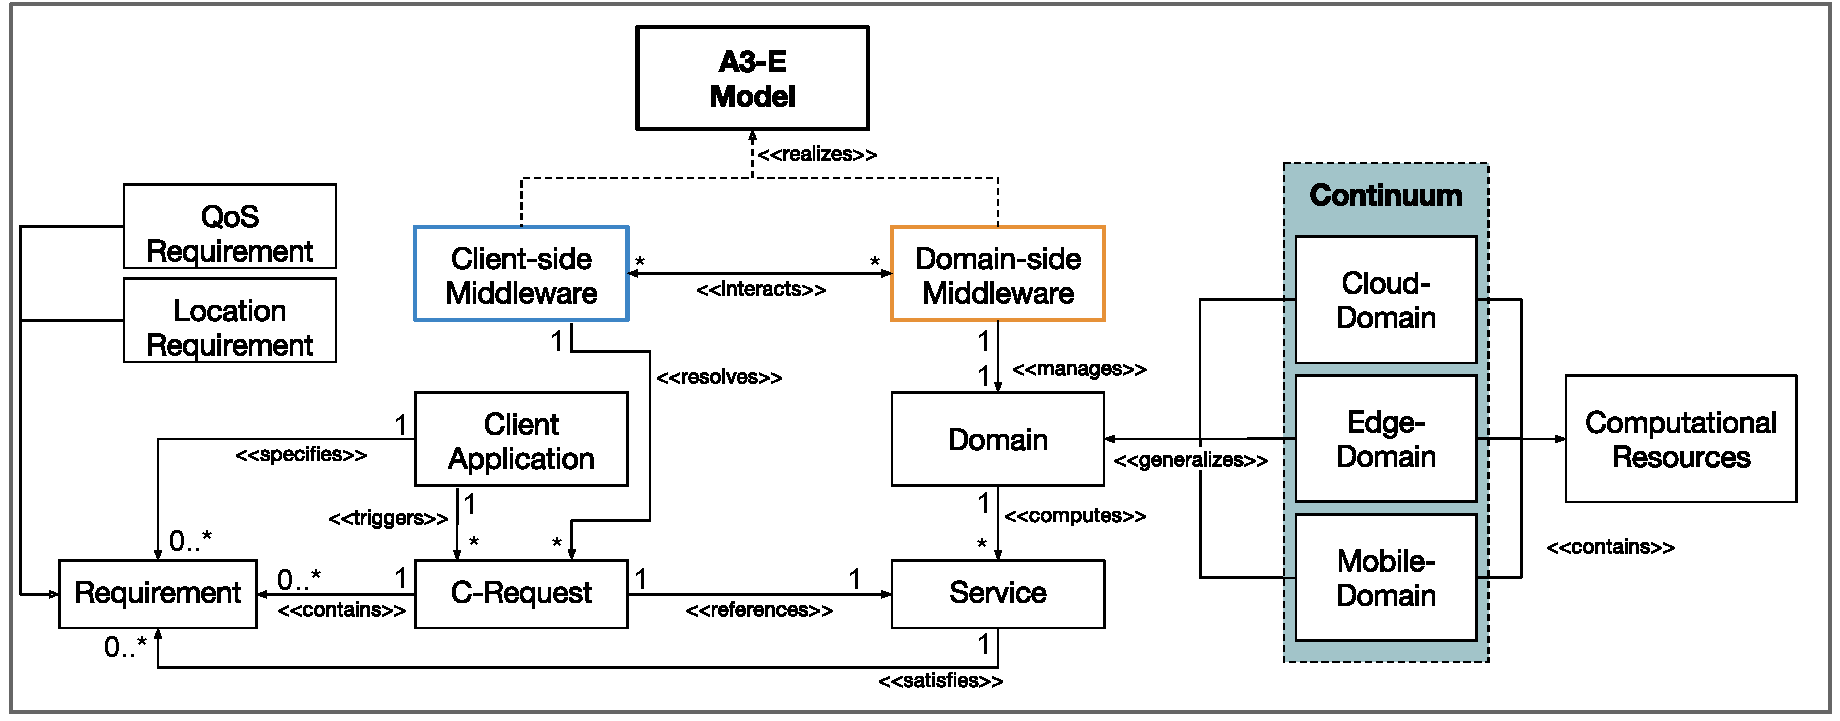
\includegraphics[width=1\textwidth]{figs/A3-E-model.pdf}
%	\caption{The Continuum Model.}
%	\label{fig:Continuum-model}
%\end{figure}

%The \textit{Continuum model}, depicted in Figure~\ref{fig:Continuum-model}, defines the actors and mechanisms involved in the realization of the mobile-edge-cloud continuum.

%Domain formalization
%Application Requirements
%Service SLA
%Service Life-cycle

\subsection{Physical Model}

%Although the continuum can hypothetically support any number of heterogeneous infrastructures, this paper focuses on three domains. The \texttt{mobile domain} is deployed to the client's mobile device, and provides local stateless computation (while enabling device-to-device collaboration through distributed mobile domains --i.e., by allowing a client to call a microservice deployed on another mobile device-- is surely interesting, for now we consider it part of our future work). The \texttt{edge domains} refer to edge-based infrastructure that can be deployed to a local server (local-edge domain) or to cellular stations (mobile-edge domain). Finally, the \texttt{cloud domain} refers to a cloud-based solution such to AWS Lambda.

%The continuum is composed of computational resources from cloud, edge, and mobile computing devices. 
%
%Cloud datacenters count with virtually unlimited computational resources needed to cope with the aggregated demand from a wide coverage area. Edge nodes~\cite{}, in contrast, are limited in computational resources, but cover a much narrower area with lower aggregated demand. 
%
%Cloud datacenters are reachable through multiple hops of network, including the Internet backbone. Edge nodes, in turn, are ideally placed a few hops away from clients to minimize network latency and jitter. 

%TODO [Martin] I've slightly changed this and next paragraph to be compliant with the ETSI standard
In our formulation, edge nodes are distinguished after the networking technology they use: \textit{mobile edge} hosts (in the context of Multi-Access Edge Computing or MEC~\cite{etsimec16,ahmed2016isco}) integrate with cellular network infrastructure (e.g., a 5G base station), whereas \textit{local edge} ones integrate with local area network infrastructure (e.g., an access point). Also, we assume that cloud and edge providers may be different from each other, and that communication among heterogeneous (mobile) edge systems~\cite{etsimec16} may not be feasible.% and unable to coordinate the allocation of resources.

%Later on, this heterogeneity is addressed with variations of the proposed service life-cycle management.

Mobile devices play two roles, namely clients and potential providers of computational resources. The motivation for including mobile devices' own resources in the model is threefold: (i) the substantial increase in computational capacity exhibited by modern devices; (ii) the compatibility of these devices with the computation of continuum microservices (see Section~\ref{sec:application_model}); and (iii) to give mobile applications a zero network latency and highly available alternative to cloud and edge providers. 

%TODO fix Figure X
%Figure X~\ref{fig:topology} illustrates a topology composed of cloud, mobile-edge, local-edge, and mobile \textit{domains}. 
Throughout this paper, we refer to \textit{cloud}, \textit{edge}, and \textit{mobile} \textit{domains}. 
%Each part of the continuum topology (cloud, mobile-edge, local-edge, and mobile) is composed of domains.
A domain yields a common  abstraction for the heterogeneous compute, storage and network resources (e.g., server(s), virtual machine(s), container(s), memory, CPU, storage, etc.) composing the continuum topology. In the particular case of MEC, the term \textit{domain} extends the one provided by ETSI for a \textit{mobile edge host}~\cite{etsimec16}.



%constituents of the continuum. Indeed, it hides the fact that they make use of heterogeneous \textit{computational resources} (e.g., server(s), virtual machine(s), container(s), memory, CPU, storage, etc.) and networking infrastructures (e.g., access points, radio access networks, etc.). 

%Examples of A3-E domains are \textit{cloud domains}, i.e., cloud-based FaaS platforms covering a specific geographical region (e.g., AWS Lambda\footnote{\url{https://aws.amazon.com/lambda}} in Europe); \textit{edge domains}, representing local-edge (e.g., domestic servers or within an office building) and mobile-edge sites (e.g., servers at cellular base stations~\cite{beck2014mobile}); and \textit{mobile domain} representing a client device's own resources.

%TODO


%Whilst cloud and edge resources are shared among different applications and managed by cloud/edge providers, mobile device resources are exclusively employed by local applications. 

\subsection{Application Model}\label{sec:application_model}

\begin{figure}[tbp]
	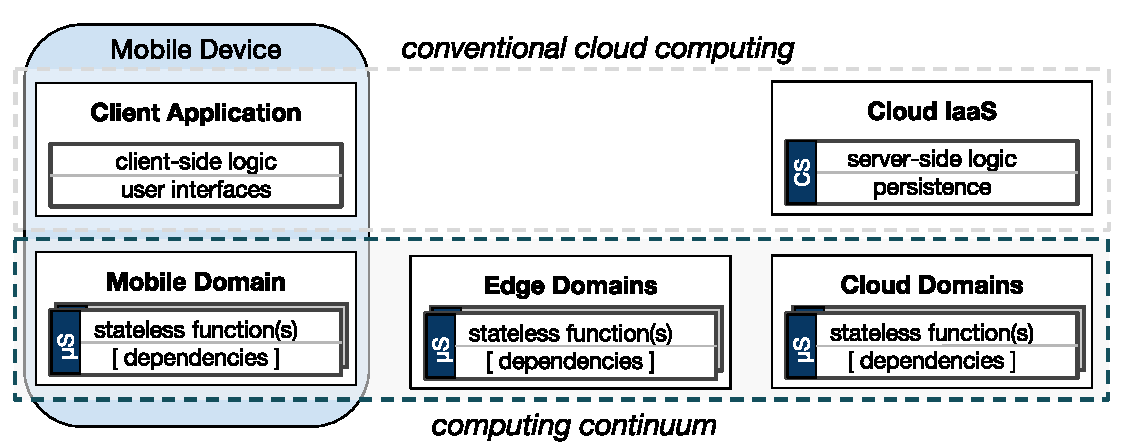
\includegraphics[width=0.85\textwidth]{figs/Continuum-arch}
	\setlength{\belowcaptionskip}{-10pt}
	\caption{The high level architecture of a mobile application exploiting both the computing continuum -- by means of $\mu$-services ($\mu$S) provided by mobile, edge, and cloud domains -- and conventional mobile/cloud computing -- by means of local computation and cloud services (CS).}
	\label{fig:Continuum-arch}
\end{figure}

On top of the physical model, we propose an \textit{application model} in which stateless components and immutable data composing \textit{continuum services} are dynamically placed to mobile, edge, and cloud,
whilst 
stateful components are deployed to cloud datacenters or the client device itself based on design-time decision.

Continuum services consist of a set of artifacts that fulfill a given functionality. In particular, these artifacts can refer to: (i) stateless function(s) (e.g., a Java compiled class); (ii) immutable data (e.g., a trained neural network model); and (iii) other dependencies (e.g., software libraries).

A priori, continuum services are portable, unless they require capabilities that can not be met by specific domains. Like cloud and edge domains, mobile domains also expose functionality by means of a well-known interface --- for the sake of consistency, the service abstraction is employed within all domains.

The proposed service model enforces data consistency and allows multiple service instances to coexist along the continuum. Also, service instances may be deployed and undeployed independently without the need for state migration, favoring the seamlessly transition from one service provider to the other. The latter is particularly important to cope with the mobility of clients. 

Continuum services are also aligned with the \textit{Function-as-a-Service} (FaaS) execution model~\cite{MateosFaaster17}. FaaS has been proposed as an alternative cloud paradigm in which business functionality is provided without pre-allocating computational resources. Instead, shared resources (e.g. containers) are used to provision and execute functions on demand, in only a few milliseconds. 

Services implemented after the FaaS model are \textit{microservices}\footnote{Hereafter referred as $\mu$-service}~\cite{lewis2014microservices}, as they are small, modular, communicate with lightweight mechanisms (often through an HTTP RESTful API) and are independently deployable by fully automated machinery. Note that our approach targets application-level functions, whereas Virtualized Network Functions (VNFs~\cite{etsimec16}) are considered as a part of the underlying infrastructure.

%This requires to support FaaS not only at cloud level, but also to bring it to (mobile) edge platforms~\cite{etsimec16}. 



As state is a fundamental aspect of many applications, we propose that mobile devices and, for most cases, cloud datacenters should remain responsible for stateful components such as persistence. This choice prevents the consistency problems (and the corresponding complexity of potential solutions) that would arise if databases were deployed to finely distributed edge nodes. %This decision is also aligned with the limitations in computational resources of edge nodes. %Indeed, the deployment of components like databases to the edge would be unrealistic for large scale applications.

%TODO: make it more general, as some applications may have local persistence and u-services may also deal with business logic
Figure~\ref{fig:Continuum-arch} illustrates the architecture overview of a continuum application. The client-side application comprises \texttt{client-side logic}, \textit{local persistence}, and \texttt{user interface} components, whereas the cloud infrastructure comprises \texttt{server-side logic} and \texttt{persistence} components. Continuum $\mu$-services are responsible for stateless computation opportunistically deployed to different domains.

\subsection{Life-cycle Management Challenges}

% [Danilo] It's been really hard to change the formulation without falling in the trap of not been objective. For me, Awareness is mostly about letting domains to know *when* to allocate resources and to let clients to know *which* domains can be chosen. Please let me know if you have insights about it. For sure I agree to make the formal part easier to digest, but it wouldn't change the focus on allocation/placement. 

The management of continuum services life-cycle is focused on two conflicting goals: i) the satisfaction of application requirements (e.g., maximum service latency, battery consumption, availability); and ii) the optimization of resources allocated for the applications. 

Dynamicity is a fundamental aspect in the continuum as mobile clients are likely to enter and exit areas covered by distinct edge domains. The aggregated demand served by cloud domains should also expect considerable variations. In any case, it may be unfeasible to predict when and how intense the demand from different applications and users will be. 

From the providers' perspective, an optimal allocation of its (virtualized) resources corresponds to the minimum number of $\mu$-service instances that must be allocated by each of its domains to cope with the SLA of each provided $\mu$-service. To be efficient, the allocation of resources should be able to mimic the corresponding fluctuations of demand, i.e., to be highly responsive. For that matter, it is important that the mechanisms governing resource allocation from each domain to be \textit{aware} of actual and potential demand for its provided $\mu$-services. 

% (e.g., maximum service latency, simultaneous request threshold, etc). 


%Even if emerging network technologies could be employed to route traffic from one base station to the other, continuum $\mu$-services implemented after the FaaS model are ephemeral (they may even last for only one invocation), stateless, and scaled as needed~\cite{Roberts:2016}. 

%In FaaS, functions are ephemeral (they may even last for only one invocation), stateless, and scaled as needed~\cite{Roberts:2016}. 

To better express this problem, let's consider the set of $\mu$-services $S = \{s_j \mid j = 0,1,...,J\}$.
%In turn, $F_i = \{f_{i,j}\}_j$ defines the set of instances of $s_i$, with $0 \le j \le n_i$.
%Instances for each $\mu$-service are defined by the set $F_i = \{f_{i,j}\}_j$, with $0 \le j \le n_i$.
Vector $\bar{c} = (c_1, ..., c_J)$ holds the number of instances for all $\mu$-services. Each instance is bound to a container; resources allocated to each container 
%Each $s_j \in S$ has a corresponding set of instances $F_j = \{f_{j,i} \mid i = 0,1,...,I_j\}$, where each instance is bound to a container. 
(e.g., CPU and memory) are considered fixed and equal for all $\mu$-services, coherently to the architecture of FaaS frameworks such as OpenWhisk~\cite{OpenWhisk}.

Now let's consider that each provided $\mu$-service $s_i \in S$ is bound to an SLA specifying its maximum service delay $\Delta_j$ and the maximum/minimum number of instances $Imin_{j}/Imax_{j}$, so that $\forall s_j \in S, Imin_j \le c_j \le Imax_j$. %, and a relative priority $p_i$. 
Given the fluctuations in the workload and the perceived delay $\tau_j$ of each service $s_j \in S$, the aim of a \textit{domain manager} is to assure that $\forall s_j \in S, \tau_j \le \Delta_j$.

Last but not least, if we consider a plethora of disjoint domains able to host the execution of $\mu$-services, each domain must be able to autonomously manage operational aspects such as the \textit{download and deployment} of $\mu$-services from new applications. 

%Also, each instance $f_{ij} \in F_i$ is bound to a single core container with fixed memory and storage. Considering that CPU is a scarcer resource, we may assume, without loss of generality, that the number of $\mu$-instances per domain is limited by the amount of CPU cores available ($|C|$) in its pool of resources, i.e., that $\sum_{i=1}^{m} k_i \le |C|$.

%Furthermore, as the demand for different services is expected to change over time, unless $\forall S_i \in S, U_i = U_i$, idle resources may be employed to reduce $\delta_i$ according to $P_i$.

From the client's viewpoint, the challenges for the materialization of the continuum are mainly twofold: i) surrogate edge domains may need to be dynamically discovered; ii) the client may need to choose among different domains able to provide similar $\mu$-services.

For a continuum application, an optimal domain selection is the one that, given a set of requirements and the perceived QoS of different services, satisfies the multi-criteria decision of which provider to be employed. Moreover, since continuum $\mu$-services are modular and independently deployed, it consists of individual decisions regarding each $\mu$-service consumed by the application.

To better express the client-side selection, let's extend the previous formulation by considering a set of independent provider domains $D = \{d_p \mid p = 1,2,...,P\}$. Each domain $d_p \in D$ provides a set of $\mu$-services $S_{p} = \{s_{p,i} \mid i =  0, 1, ..., I_p\}$. In turn, a continuum application $CA_x$ relies on the set of $\mu$-services $S_x = \{s_a \mid a = 1,2,...,A\}$, so that $\forall s_a \in S_x$, there is at least one provider domain offering that $\mu$-service, that is, $\forall s_a \in S_x, \exists\ s_{p,i} \in \bigcup_{p=1}^{|P|} S_p \wedge s_{p,i} = s_a$. 

Now let's consider that each $s_a \in S_x$ is bound to a set of required QoS attributes $QoS_a = \{qa_u \mid u = 0, 1, ..., U\}$ and that each $qa_u \in QoS_a$ is represented by a tuple $(constraint_u, weigth_u)$ respectively defining the an expression (e.g. response time < 300ms) and weight for that attribute. For each $qa_u \in QoS_a$, $actual_{p,a,u}$ defines the value for that QoS attribute as perceived by the client. It follows that, for each $s_a \in S_x$ from application $CA_x$, the aim of the \textit{mobile middleware} is to select the domain $d_p \in D$ 
%best satisfying the set of attributes in $QoS_o$, i.e., 
that maximizes the utility function $U(p) = \sum_{u=1}^{U} weigth_u * actual_{p,a,u}$, provided that $\forall qa_u \in QoS_a, actual_{p,a,u} \vdash constraint_u$.

%service latency and cost as our requirements. From the client viewpoint, latency can be refined into network and service latency, with cloud providers exhibiting highest network latency and lowest service latency due to more powerful computational power; edge providers exhibiting low network latency and higher service latency; and finally the local mobile environment exhibiting zero network latency and the highest service latency due to more limited computational power. Service cost, in turn, is lower in the cloud than in the edge and null in the mobile environment. Given the relative importance of each attribute, the aim of the provider selection is to 


%The life-cycle management is therefore dual: it comprises the provider-side allocation of service instances at each domain; and it also encompasses the client-side decision of which domain must be selected for each continuum $\mu$-service.

\subsection{Running Example}
\label{sub:example}

\begin{figure}[tbp]
	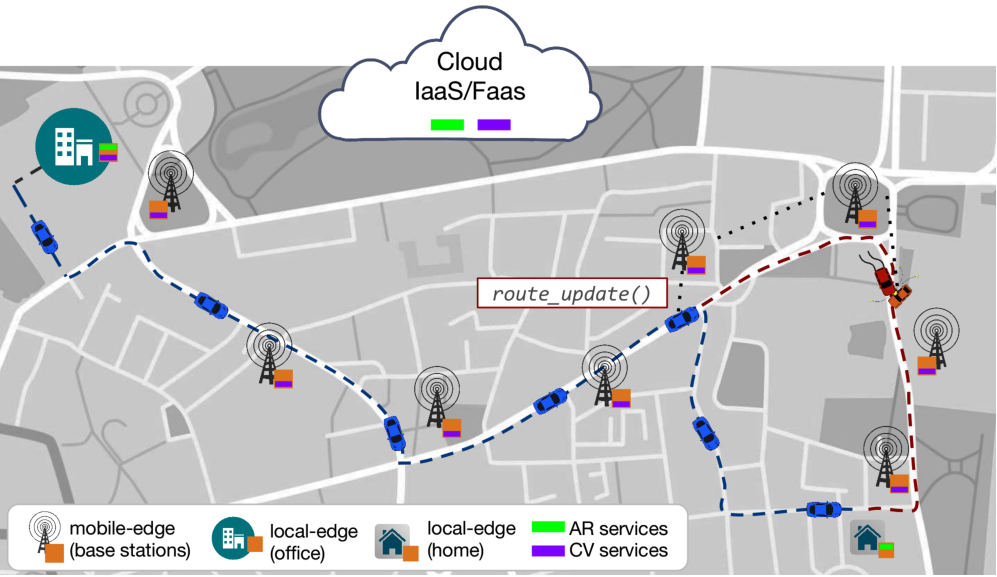
\includegraphics[width=0.7\textwidth]{figs/Continuum-Scenario}
	\setlength{\belowcaptionskip}{-8pt}
	\caption{Heterogeneous applications such as Augmented Reality and Mobile Games (MG) rely on $\mu$-services deployed along the compute continuum (mobile, mobile-edge, local-edge, and cloud).}
	\label{fig:continuum-scenario}
\end{figure}

%Figure~\ref{fig:continuum-scenario} shows a complete example scenario involving different applications that rely on computation executed in the cloud, edge, or in the user's own devices.

We illustrate the continuum with an example scenario involving different applications that rely on computation executed in the cloud, edge, or in the user's own device.

First, let us consider an Augmented Reality (AR)~\cite{GarrigaMendonca2017} application employed by our user to 
explore the points of interest (POI) in the touristic areas from the city she is currently visiting.
%craft virtual 3D objects that are added to her \textit{smart glasses} as part of her work. 
This real-time application involves heavyweight image processing for the \textit{extraction of features} from the captured scenes, as well as a trained neural network model to \textit{match features} from an extensive object catalog. Given its requirements for augmentation and computation offloading, this is an application class that can benefit from the adoption of the continuum~\cite{beck2014mobile}.

Two continuum $\mu$-services are modeled after each task: one relies on a image processing library and a trained model, the other on a feature-based object catalog. Client-side logic is responsible for capturing scenes from the glasses' camera and updating the 3D virtual object in the scene rendered by the smart glasses.

Despite the capacity of existing smart devices (e.g., Glass~\footnote{https://x.company/glass/}) in hosting a plethora of applications, the user may experience functional and non-functional degradation (e.g., reduced object catalog, battery drain, etc). With the offloading of the aforementioned tasks to a server, the user can enjoy an improved Quality-of-Experience.

%avoid recharging her glasses and improve productivity. 

To support this and other applications, mobile-edge servers were deployed to the base stations covering touristic areas. Their additional storage allows a larger set of objects to be recognized, thanks to a more completely trained model. Variations in the workload are handled with a fast instantiation of $\mu$-services, which must consider other applications relying on the same servers.

%In contrast, the network latency to cloud servers may be prohibitive for this real-time application. The decision of which continuum provider to employ must be informed by the application requirements and the Quality-of-Service (QoS) of each alternative. 

After her tour, our user calls for an autonomous vehicle (AV) to drive her back to her hotel. During the way, she starts editing the pictures taken that day, activity interrupted only by eventual notification from the AR application showing nearby POI information. 

To reduce processing time and avoid battery drain, the AV features a local-edge server that provides a catalog of $\mu$-services for image processing, including those of the AR. Meanwhile, the vehicle makes use of a \textit{route planning} $\mu$-service
%deployed at mobile-edge servers located at cellular base stations 
%to receive updates about 
to calculate the best plan to reach our user's destination. Since latency is not a main requirement, the latter is served by a cloud provider whenever the AV's local-edge resources are not available. 

%Additionally, it relies on low-latency services to become aware of sudden events like accidents.

%To support the AV, two continuum $\mu$-services are envisioned: the \textit{route planning}, which relies on a traffic dataset and a routing software and can cope with higher latency, and the \textit{incident notification}, which relies on low-latency communication between vehicles and mobile-edge base stations to forward incident events received by that base-station.

%TODO: the incident notification is not consistent with our service model; either remove the AV example or find a different kind of low-latency service (e.g., augmented reality of what is seen from inside the car?)
%[Danilo] What about web sockets? Or push-notification? 

%within milliseconds the vehicle can become aware of to adjust its routes to avoid heavy traffic. In particular, let's say that a new path consists of residential streets with data services only (without mobile-edge coverage). The AV continues to fetch updates, which are now served by a cloud provider. The additional network latency is partially compensated with the low speed limit of the residential area.

%During our user's journey home, her AV passes by a touristic region. The mobile-edge domains covering this area provides continuum $\mu$-services to be consumed by an AR application for tourists. These services share computational resources with those of AVs passing by the same area, as well as any other continuum $\mu$-services that happens to be provided by those mobile-edge domains.

%Due to resource limitation, each mobile-edge domain must employ mechanisms to efficiently manage its resources and assure that competing $\mu$-services are best provided according to their Service Level Agreement (SLA). In our example, the AV's \textit{incident notification} $\mu$-services is likely to enjoy a higher priority regarding the AR's $\mu$-services due to the criticality of the former.

Finally at her hotel room, our user 
%can start using her domestic local-edge. She 
continues with the image and video editing. Later on, she decides to enjoy a Mobile Game (MG) application. The MG consists of client-side logic and
user interfaces (e.g., controllers and views of an MVC\footnote{Model-View-Controller architectural pattern}). In particular, the game model features complex calculations that pose a burden to her mobile device's CPU. 
%The application consists of for processing the game state, which must be passed as a parameter in conjunction with game events (e.g., user inputs). 

Supporting guest applications, the hotel provides a local-edge server. The latter identifies the image editing and the MG applications and, upon download and installation, starts providing the required $\mu$-services. %for processing the game state, which must be passed as a parameter in conjunction with game events (e.g., user inputs). 
Last but not least, conventional cloud services provide stateful services (e.g., multimedia storage, game authentication, player scores, etc).% and persistence (e.g., player scores).  

%This latter scenario exploits different parts of the continuum. A domestic local-edge domain must identify, fetch, and deploy the corresponding $\mu$-services. Meanwhile and to assure a high availability, the mobile domain remains responsible for the provisioning of these $\mu$-services. Finally, cloud domains complement the possible alternatives for hosting the $\mu$-services and mitigating battery drain, but network latency must be taken into account.

%Traditional cloud resources are employed as a reliable alternative to edge-based computation. Similarly, local services are employed as alternatives to edge services until they have been acquired and made available by a local-edge server. Whilst the transition between mobile-edge and cloud is transparent, the use of local-edge services involves mutual client-server awareness.


%TODO [Danilo] better in proposal
%Upon installation, the local-edge server becomes aware of a new continuum-compliant application and, while the app continues to run locally on her device, it proceeds to setup the services needed to allow the application to offload some of the computation. Once the setup is complete, the application autonomously starts using the edge services with the purpose of preserving the device's resources. Not only does the game's performance improve, battery consumption is also reduced.  





	\section{A3-E}\label{sec:A3-E}

%\begin{figure}[tbp]
%	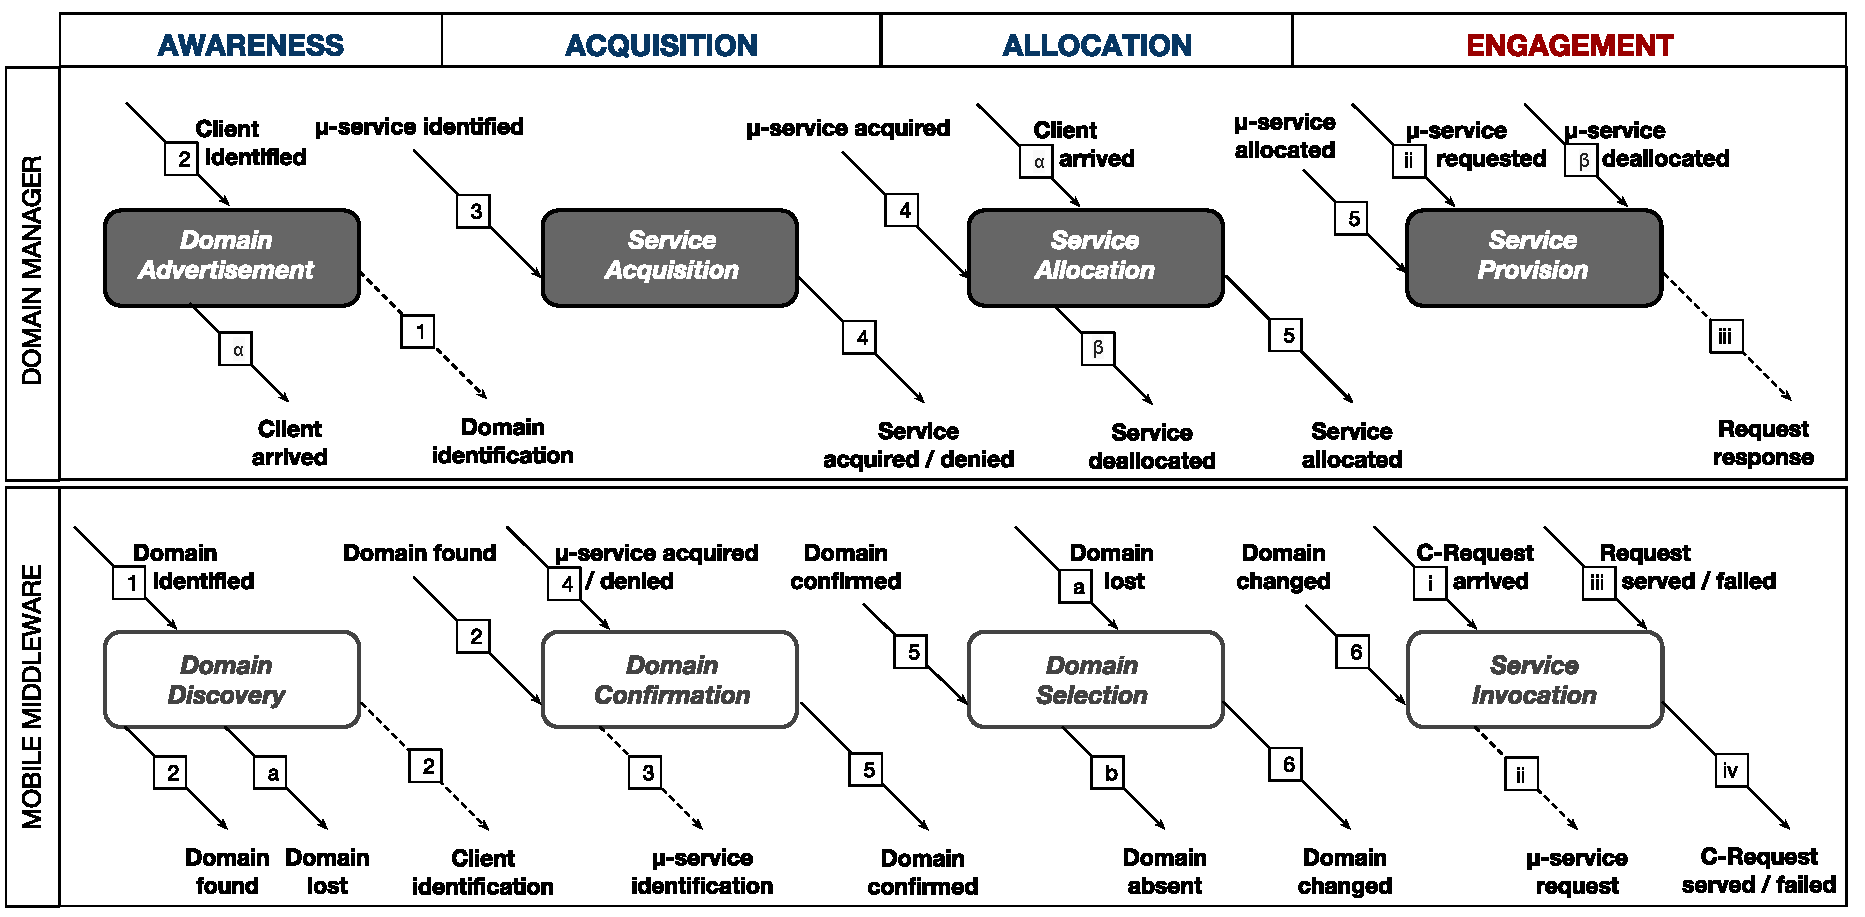
\includegraphics[width=0.92\textwidth]{figs/A3-E-process}
%%	\setlength{\belowcaptionskip}{-10pt}
%	\caption{A3-E overview. A3-E's activities are carried out by a \textit{domain manager} and a \textit{mobile middleware}, and coordinate through incoming ($\rightarrow$) and outgoing ($\leftarrow$) asynchronous events.}
%	\label{fig:A3-E-process}
%\end{figure}

\begin{figure}[tbp]
	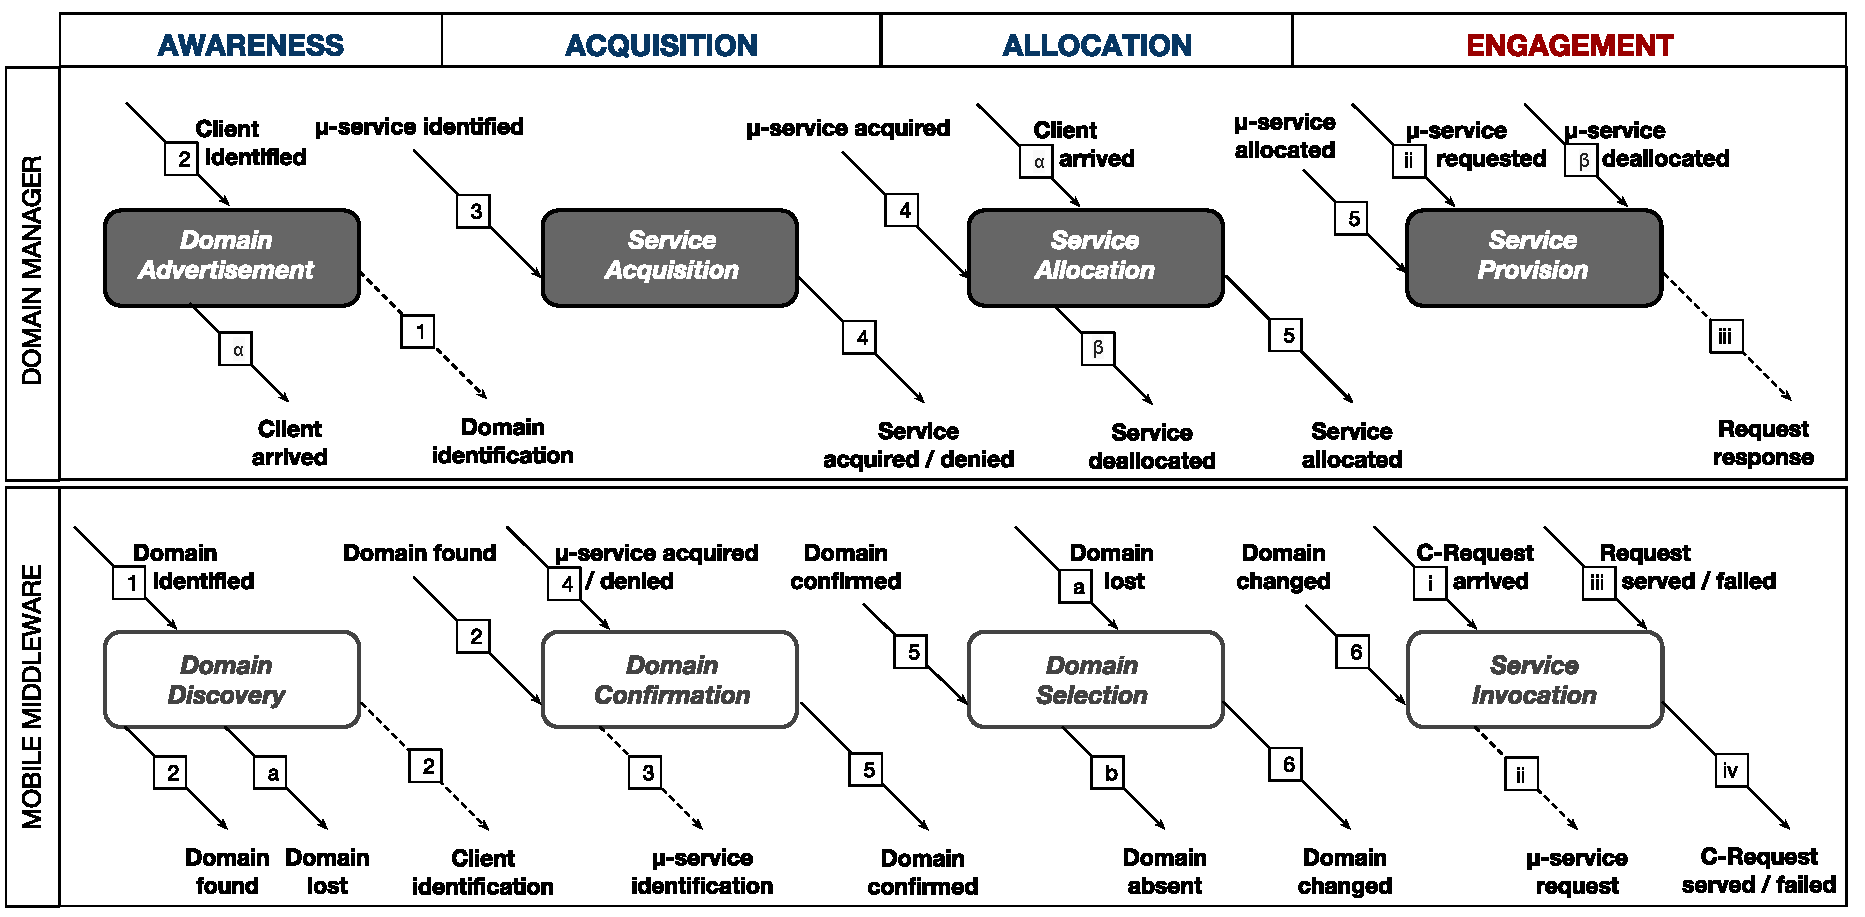
\includegraphics[width=0.85\textwidth]{figs/A3-E-process}
	%	\setlength{\belowcaptionskip}{-10pt}
	\caption{A3-E overview. A3-E's activities --- (AW)areness, (AQ)uisition, (AL)location, (E)ngagement --- are carried out by a \textit{domain manager} and a \textit{mobile middleware}, and coordinate through asynchronous events depicted by and identified as follows: \textit{domain identification}~(DI), \textit{client identification}~(CI), \textit{client arrived}~(CA),\textit{client left}~(CL),\textit{$\mu$-service identified}~($\mu$I), \textit{$\mu$-service acquired}~($\mu$AQ), \textit{$\mu$-service allocated}~($\mu$AL), \textit{$\mu$-service (deallocated}~($\mu$DA), \textit{domain found}~(DF), \textit{domain lost}~(DL), \textit{domain ready}~(DR), \textit{domain changed}~(DS), \textit{execution time}~($\Delta$EX), \textit{$\mu$-service request}~($\mu$RQ), \textit{$\mu$-service response}~($\mu$RS), \textit{C-Request}~(C-RQ).}
	\label{fig:A3-E-process}
\end{figure}

%First and foremost, A3-E's main objective is to enable the efficient and scalable placement of $\mu$-services along the continuum. In A3-E, clients and providers autonomously interact and decide for the placement of services according to the context. Moreover,  

To realize the mobile-edge-cloud continuum, we propose A3-E, a model supporting the self-management of continuum $\mu$-service life-cycles. A3-E inherits its name from its four main activities -- namely, \textit{(\textbf{A})wareness, (\textbf{A})cquisition, (\textbf{A})llocation, and (\textbf{E})ngagement}. 

A3-E targets 
the efficient and scalable placement of $\mu$-services along the continuum and the satisfaction of application requirements such as maximum service latency, battery consumption, and availability. 
To achieve it, clients and heterogeneous domains take part in the automated and opportunistic decision of which continuum resources --- among those of mobile, edge, and cloud --- should be employed in provisioning each of the $\mu$-service required by continuum applications. 

%A3-E targets 
%%the materialization of the continuum by means of an
%the efficient and scalable placement of $\mu$-services along the continuum. 
%To achieve it, clients and heterogeneous \textit{mobile, edge, and cloud} domains take part in the \textit{automated} and \textit{decentralized} decision of which continuum resources should be employed in provisioning each of the $\mu$-services required by continuum applications.% according to the context of operation.


%A3-E exploits the FaaS paradigm and propose additional mechanisms for 

Figure~\ref{fig:A3-E-process} illustrates each activity in A3-E. 
Activities are refined by procedures that coordinate through asynchronous events and are carried out by a \textit{domain manager} and by a \textit{mobile middleware}. 
%Activities from both sides are coordinated through signals and events. 
To address the intrinsic heterogeneity of the continuum, A3-E is flexible with respect to how each of its activities is actually implemented. 
%For each phase, the main activities of a \textit{domain} and a \textit{client} are depicted along with their mutual relative state at the moment the phase starts: for a domain, a service state ranges from \textit{Free} to \textit{Allocated}, whilst a domain state ranges from \textit{Away} to \textit{Selected} for a client. 
%More precisely, Fig.~\ref{fig:A3-E-process} refers to the activities and states (in parenthesis) of a single client-domain interaction.

%Next, we detail each main activity in A3-E, starting from the most general one, i.e., the one that applies to all types of client-domain interaction, and moving towards the more specific ones.


%\subsection{A3-E Process: Phases}\label{sec:A3-E-process}

%Next, the four A3-E phases are further described and mapped to the requirements elicited in  Section~\ref{sec:requirements}. Later on, other possible instances of the A3-E model are correlated with scenarios of the compute continuum.


\subsection{Awareness}\label{sec:A3-E-awareness}

%From the provider's viewpoint, the main purpose of Awareness is to enable domains to opportunistically and pro-actively initialize the Acquisition and Allocation activities. %, based on the awareness of devices in a domain's coverage area. 
%In turn, clients benefit from Awareness with the dynamic discovery and profiling of domains that can provide the $\mu$-services they need.

%A3-E's Awareness models (i) the discovery of domains and (ii) the discovery of continuum applications in one of its domains' area of coverage, indicating the imminent need for specific $\mu$-services. 




The latency of continuum $\mu$-services can be decomposed into three parts: \textit{acquisition delay} ($\Delta AQ$), \textit{allocation delay} ($\Delta AL$), and \textit{execution delay} ($\Delta E$). FaaS platforms like AWS Lambda~\cite{AWSLambda}
%~\footnote{https://docs.aws.amazon.com/lambda/latest/dg/running-lambda-code.html}
and OpenWhisk~\cite{OpenWhisk} adopt a \textit{cold start} policy in which $\mu$-services are allocated after their first call following a period of idleness. This latency, however, may be disruptive for some applications. 
%To satisfy the maximum accepted latency of provided $\mu$-services, a \textit{domain manager} mitigates each component as follows: 

%In comparison, %the proposed mutual client-provider awareness 
A3-E's Awareness has two benefits: (i) it alleviates $\Delta AL$ (cold starts) by pro-actively allocating $\mu$-services just before they are needed; and (ii) it reduces $\Delta AQ$ and enables $\mu$-service acquisition to be opportunistic (i.e., on demand) by triggering the download and installation of new $\mu$-services as soon as the client becomes active in a specific domain (e.g., by starting the application or by entering an edge domain's area).

%TODO [Danilo] this kind of detail fits better in the implementation, doesn't it?
While cloud domains are not likely to change, and may be set-up statically by clients,% to realize this activity
edge domains must advertise their existence (\textit{domain identification}) using protocols that are compatible with its network infrastructure: for instance, through IP broadcasting in local-edge, and through Evolved Multimedia Broadcast/Multicast Service (eMBMS) in mobile-edge~\cite{lecompte2012evolved,etsimec16:03}. 
In particular, edge domains exploit locality by triggering a \textit{client left} event once mobile devices leave its coverage area, whilst cloud domains rely on adjustable \textit{timeout}.% for triggering this event.




%Throughout Awareness, the domain manager handles the following event:

%{\small
%\begin{itemize}
%	
%	\item \textbf{Client identified:} triggered when a new client enters the domain's coverage area. The manager must react with the triggering of a \textit{client arrived} and \textit{$\mu$-service identified} events for each $\mu$-service required by the client.
%	
%\end{itemize}
%}%

From the client's perspective, Awareness corresponds to the discovery of domains (source of \textit{domain found} and \textit{domain lost} events) and the advertisement of required $\mu$-services through a \textit{client identification} signal containing their metadata (name, repository url), upon which the domain manager triggers both \textit{client arrived} and \textit{$\mu$-service identified} events.% for each required $\mu$-service. 

To realize this activity, special purpose HTTP endpoints can be used for cloud domains; protocols from local area networks (e.g., UDP, IP multicast) are used for local-edge domains; eMBMS protocols (e.g., FLUTE~\cite{lecompte2012evolved}) which are carried over traditional UDP and IP multicast toward end-user devices, are used for mobile-edge domains; and system-level signals (e.g., broadcast intents in Android platforms) are used by mobile domains.

%[Danilo] 2ndR: this paragraph is poor
%In our running example, the mobile-edge and local-edge domains must advertise their existence to our user's device, which in turn identifies the AR and Image Editing applications. The same holds for the hotel's local-edge domain and the MG application. %In all cases, cloud and edge domains can employ Awareness to opportunistically fetch, install, and allocate instances of required $\mu$-services.


%The mobile middleware, in turn, realizes Awareness with the discovery of cloud and edge domains. In particular, 
%During Awareness, the mobile middleware handles the following event:
%
%{\small
%\begin{itemize}
%	
%	\item \textbf{Domain identified:} triggered when a domain is found. The middleware must react with the triggering of a \textit{domain found} event and a \textit{client identification} signal to the domain manager.
%	
%\end{itemize}
%}%

%To implement Awareness, 

%It copes with the need for efficiency and scalability of finely distributed edge domains by allowing acquisition and/or allocation of services to happen just in time, i.e., just before the client application needs them.
%and enables not only functions to be allocated, but also acquired in an opportunistic fashion.
%The benefit lies in the anticipation of (opportunistic) services setup with respect to the arrival of the first service request, i.e., in the mitigation of service setup delay (also known as cold start). Since cloud domains cover a large area, the later do not employ the awareness phase. Needless to say, mobile domains do not require awareness for sharing the same platform with client applications.

%TODO [Danilo] Commented-out in favor of a more abstract description in terms of events, as broadcasting is something local-edge specific
%The DSM achieves this by broadcasting its existence and by waiting for clients to pass along their requirements. In our running example this occurs when the user's domestic local-edge server becomes aware of the new mobile game that the user had just installed. 
%%nd the discovery of client applications along with their requirements (i.e., services). The later are passed to the following phase of acquisition.
%%then receive all client application requirements (i.e., services) as soon as the client's mobile device enters the domain's coverage area, and then pro-actively starting acquisition and allocation. 
%%For example, in the real-time translation application previously introduced, the service setup delay was mitigated by having the acquisition of the data and codebase composing the service to start as soon as the user entered the edge domain's coverage area.
%%For example, the setup of services required by the mobile multiplayer game application by the user's local-edge server follows the awareness of a new application.
%From the client's perspective, the awareness phase models the discovery of domains, and corresponding $\mu$-services, whose network addresses are not previously known. In particular, it tackles edge domains that are integrated with the local network infrastructures of buildings and public spaces. This modality contrasts with cloud which are accessed through DNS and traffic managers. Needless to say, the awareness phase is not considered by mobile domains. The CSM intercepts the provider's broadcast messages, and reacts by sending back its application requirements. This process should happen once, and in a timely fashion, upon connection to new networks to mitigate battery consumption. As an example, the local-edge server in our user's home is discovered when her mobile device connects to her domestic Wi-Fi network. 


%Once the domain is ready, this domain becomes an alternative for the provisioning of services required by the many applications (e.g., the mobile multiplayer game) hosted by the user's smartphone, tablet, and/or other of his IoT gadgets. 


%Finally, the Awareness phase has the following purposes: 1) to enable domains to pro-actively initialize the acquisition and allocation phases based on its awareness of applications whose hosting devices happens to be in the domain coverage area (Req.~\textbf{R2.3}); and 2) to enable clients to discover the address of local domains (Req.~\textbf{R2.2}).

%From the domains perspective, the awareness of clients presence in their coverage area allows a proactive download and installation of services artifacts (acquisition phase) and/or the allocation of services (allocation phase) potentially before a first request to that service arrives, alleviating the delay introduced by services setup.  From the clients perspective, the awareness phase increases the range of alternatives from the continuum that can be used to satisfy their requirements.

%Such behavior allows that are opportunistically acquired and/or allocated to mitigate their setup delay by triggering these phases upon awareness of client(s) in their coverage area.

%From the domain-side, the lack of awareness of clients in the domain coverage area prevents triggering the acquisition and subsequently allocation phases based on this event. From the client-side, the lack of awareness from surrounding domains prevents them to make the decision of which domains to use. In the later case, clients must rely on external components to reach servers (e.g., traffic managers and DNS servers).

\subsection{Acquisition}\label{sec:A3-E-acquisition}

A3-E's \textit{Acquisition} models the automated download and installation of continuum $\mu$-service artifacts, and the confirmation of the domain's capability in providing that $\mu$-service. Its ultimate goal is to mitigate the use of domain resources before the $\mu$-service is actually needed, while also facilitating IT operations (Ops) for developers and administrators. 

Ops mitigation is particularly important in (finely distributed) edge domains, since the manual administration of a large number of $\mu$-services can prove cumbersome and expensive. Nevertheless, this can also prove useful for cloud domains. Indeed, to the best of our knowledge, current FaaS platforms only support uploading (pushing) functions through public interfaces. 

Acquisition is autonomously managed, therefore it allows $\mu$-services to be downloaded 
%(e.g., pulled from a repository) 
and installed on demand. A domain manager fetches the artifacts (e.g., compiled classes and dependencies) from a repository upon the arrival of a \textit{$\mu$-service identified} event. Note that mobile domains are exempt of performing Acquisition as local $\mu$-services are assumed to be downloaded and installed along with the client application and the mobile middleware. 

% In addition to function sources, artifacts may comprise data and libraries needed by the service.

%Throughout Acquisition, the domain manager handles the following event:
%
%{\small
%\begin{itemize}
%	
%	\item \textbf{$\mu$-service identified:} indicates the request for deployment of a new $\mu$-service. The manager must proceed with the download and installation of the $\mu$-service, followed by the triggering of a \textit{service acquired} (or \textit{denied}) signal/event according to the activity outcome.
%	%its capability in providing that $\mu$-service.
%	
%	%\item \textbf{Client arrived:} triggered when a new client entered the domain's coverage area. The manager must react with 
%	
%\end{itemize}
%}%

%In this phase, the domain manager receives a set of application requirements from the client's CSM, namely the list of $\mu$-services and the URL of their repositories. The desired $\mu$-service artifacts are then downloaded and installed, at which point the DSM informs the client whether the $\mu$-services can be considered ``acquired'' or not. 
%Throughout the $\mu$-services' life-cycles, the DSM periodically checks for new versions of acquired services and updates them accordingly. 
%As an example, the services consumed by both AR applications introduced early can be autonomously acquired on demand by the local-edge servers in the user's office and home, preventing the company and the user to perform such operation. 
%In case the service has already been acquired or as the acquisition finishes, clients should add that domain to their list of available domains. 

From the client's perspective, Acquisition corresponds to the confirmation (or denial) of a domain's capability in providing the $\mu$-services required by the application. After a \textit{domain found} event, the mobile middleware listens for a \textit{$\mu$-service acquired} signal --- to be handled with the update of a list of capable domains and the subsequent triggering of a \textit{domain confirmed} (or \textit{denied}) event.

In our running example, the assets composing the $\mu$-services from the AR, Image Editing, and MG applications are once fetched and installed by the two local-edge domains upon arrival of a first \textit{$\mu$-service identified} event. While this is achieved, the applications momentarily continue to rely on their own mobile domain, or on any other domain on which $\mu$-services have already been acquired and allocated due to a previous client-domain interaction (e.g., the mobile-edge domains in our example skip Acquisition of AR artifacts due to previous contact with tourist devices).

%
%During this activity, the mobile middleware deals with the following events:
%
%{\small
%\begin{itemize}
%	
%	\item \textbf{Domain found:} indicates a potential domain for a $\mu$-service has been found. The middleware must proceed with the \textit{$\mu$-service identification} signal (if the domain is new) followed by the triggering of a \textit{domain confirmed} event.	
%	
%	\item \textbf{$\mu$-service acquired:} indicates a successful acquisition of a previously identified $\mu$-service. The middleware must react with the triggering of a \textit{domain confirmed} event.
%	
%	\item \textbf{$\mu$-service denied:} indicates the failure in acquiring and/or deploying a $\mu$-service. The middleware must proceed with the blacklisting of that domain. 
%	
%\end{itemize}
%}%


 %follow the identification of the domain's capability in providing the requested service. This phase is realized by the CSM with the following sub-process: the CSM should expect a confirmation from the DSM regarding its compliance in providing the service required by the application. Once confirmed, the CSM adds that domain to a list of available domains used by the client-side allocation phase. 

%As an example, a real-time translation application from/to streams of different spoken languages require services with low-latency. The translation can either rely on local services provided by the mobile domain (zero network latency) or on remote services provided by the edge domain (low network latency). Given the battery constraints of the mobile device, edge services are preferred. Instead of having all artifacts pre-installed, the edge's DSM acquires the data and codebase from a repository informed by the CSM upon detection of the user in its coverage area. The setup process takes no more than a minute, during which local services were consumed. Once the setup is ready, the application can start streaming captured conversations to edge-based services, which in turn reply with a translated audio stream.

%From the domain-side, the lack of acquisition implies that service assets must be previously made available. Nonetheless, the preliminary acquisition of a large number of assets is limited by the domain storage capability. 

%Conversely, the automated and opportunistic acquisition of service assets improves storage efficiency with the cost of a setup time $\Delta_{AQ}$. For instance, domains that become aware of clients' requirements may pro-actively start the acquisition phase and become ready for allocation before the first service request arrives.

%otherwise, domains must rely on the detection of a first service request or some other triggering condition to start the acquisition phase and, after setup time $\Delta_A$, become ready for allocation. 



\subsection{Allocation}\label{sec:A3-E-allocation}

%\begin{figure}[thbp]
%	\centering
%	\captionsetup[subfigure]{width=0.4\textwidth}	
%	\null\hfill
%	\subfloat[Domain $\mu$-services allocation control loop; domains must monitor the QoS of deployed $\mu$-services and adapt its allocation scheme to prevent SLA violations.\label{fig:service-allocation-loop}]{ 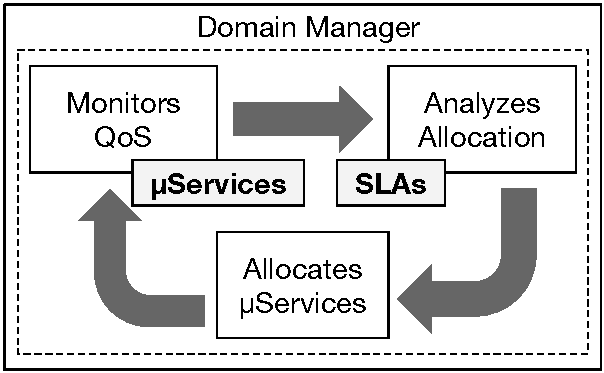
\includegraphics[width=0.4\textwidth]{figs/service-allocation-loop}}
%	\captionsetup[subfigure]{width=0.4\textwidth}	
%	\hfill
%	\subfloat[Per $\mu$-service domain selection control loop; clients monitor $\mu$-services from available domains and select the one that best satisfies its requirements.\label{fig:domain-selection-loop}] {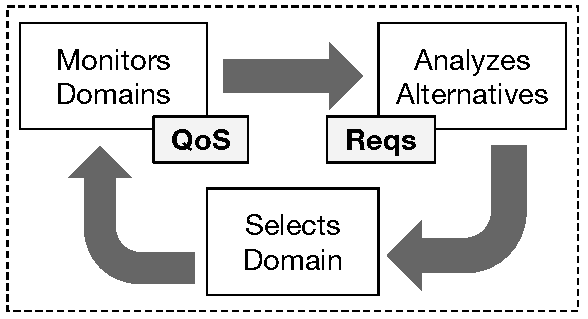
\includegraphics[width=0.4\textwidth]{figs/domain-selection-loop}}
%	\hfill\null
%	\caption{Self-management loops for domain-side $\mu$-services allocation and client-side domain selection}\label{fig:allocation-loops}
%\end{figure}


\textit{Allocation} models the deployment of continuum $\mu$-services on a pool of resources provided by the domain. It also captures the client-side selection of domains for each of the $\mu$-services employed by the application.

%From the domain's perspective, the allocation phase models the placement of $\mu$-services on the domain's resources, i.e., on its pool of servers, virtual machines, and containers. At the beginning of this phase, $\mu$-service artifacts have been \textit{acquired} by the domain, and the client has been \textit{notified} of this.

The scope of the provider-side Allocation is limited by its domain boundaries. Cloud domains allocate $\mu$-service instances to containers in resourceful datacenters covering a large area. On the other hand, edge domains rely on containers from one or more (virtual) machines serving an office or a building (local-edge) or a 5G base station area (mobile-edge). Finally, the allocation of $\mu$-services into mobile domain resources is platform specific (e.g., Android service life-cycle).

%pre-allocated and no allocation is needed.

%In this paper, we do not consider inter-domain cooperation (e.g., placement among different domains).

Existing FaaS platforms handle Allocation with on demand instantiation of containers after a first request, which may be kept \textit{warm} before being deallocated after a period of idleness~\cite{AWSLambda, OpenWhisk}. A3-E generalizes this mechanism as a self-management loop~\cite{kephart2003vision}
in which $\mu$-service instances are allocated to cloud and edge domain resources to guarantee that service latency and availability of each provided $\mu$-service are in-line with the desired SLA. 

%To better express this problem, let's consider the set of $\mu$-services $S = \{s_j \mid j = 0,1,...,J\}$.
%%In turn, $F_i = \{f_{i,j}\}_j$ defines the set of instances of $s_i$, with $0 \le j \le n_i$.
%%Instances for each $\mu$-service are defined by the set $F_i = \{f_{i,j}\}_j$, with $0 \le j \le n_i$.
%Vector $\bar{c} = (c_1, ..., c_J)$ holds the number of instances for all $\mu$-services. Each instance is bound to a container; resources allocated to each container 
%%Each $s_j \in S$ has a corresponding set of instances $F_j = \{f_{j,i} \mid i = 0,1,...,I_j\}$, where each instance is bound to a container. 
%(e.g., CPU and memory) are considered fixed and equal for all $\mu$-services, coherently to the architecture of FaaS frameworks such as OpenWhisk~\cite{OpenWhisk}.
%
%Now let's assume that each provided $\mu$-service $s_i \in S$ is bound to an SLA specifying its \textit{maximum accepted service latency} $\Delta_j$ 
%as well as the minimum/maximum number of service instances $Kmin_{j}/Kmax_{j}$. %, and a relative priority $p_i$. 
%Given the fluctuations in the workload and the response time $\tau_j$ (comprising both \textit{queue time} and \textit{service time}) of each $\mu$-service $s_j \in S$, the aim of a \textit{domain manager} is to find the minimum $c_j$ for each $\mu$-service so that, $\forall s_j \in S,\ \tau_j \le \Delta_j\ \wedge\ Kmin_j \le c_j \le Kmax_j$. 

To achieve this goal, the self-management \textit{monitor} ($M$ in Fig.~\ref{fig:A3-E-process}) calculates the \textit{arrival rate} ($\alpha_j$) and the \textit{response time} ($\tau_j$), as well as the \textit{number of clients} for each provided $\mu$-service ($s_{j} \in S$). The first two parameters are updated after each $\mu$-service execution ($QoS$ in Fig.~\ref{fig:A3-E-process}), whilst the second depends on \textit{client arrived} and \textit{client left} events from Awareness (respectively $CA$ and $CL$ in Fig.~\ref{fig:A3-E-process}). The \textit{analyzer} ($A$ in Fig.~\ref{fig:A3-E-process}) then outputs the number of instances $c_j$ for each $s_j \in S$ so that $\forall s_j \in S,\ \tau_j \le \Delta_j\ \wedge\ Kmin_j \le c_j \le Kmax_j$. It is up to the \textit{planner} ($P$ in Fig.~\ref{fig:A3-E-process}) to decide if and how to cope with the new allocation scheme based on the domain's resources (memory and CPU) and SLA for each $s_j \in S$.
%Moreover, the monitoring procedure considers the response time ($\tau_j$) and 
To mitigate \textit{cold start} ($\Delta 2_j$), the planner reacts to a \textit{client arrived} event by anticipating container allocation if resources are available at that loop iteration; and by keeping containers allocated (\textit{warm}) after a $\mu$-service execution. Finally, the \textit{executor} ($E$ in Fig.~\ref{fig:A3-E-process}) carries out the new allocation scheme by means of commands to the container platform (i.e., Docker).

%Throughout Allocation, the domain manager reacts to a 
%a \textit{$\mu$-service acquired} event --- indicating that the function(s) and dependencies have been fetched, and that the $\mu$-service is ready to be deployed ---  
%%The domain manager must react 
%by including this $\mu$-service in its self-management loop handling allocation. 
%%\textbf{THIS SELF-MANAGEMENT LOOP IS NOT WELL INTRODUCED. IT KIND OF DROPS OUT OF NOWHERE} 
%Also, to mitigate cold starts, the manager should react to a \textit{client arrived} event by anticipating Allocation for each identified $\mu$-service, if resources are available. 
%Finally, the manager should take into account a \textit{$\mu$-service requested} by updating the corresponding arrival rate metric. \textbf{I DON"T UNDERSTAND WHAT YOU MEAN HERE.}

Given the resource limitations of edge domains, contention between different $\mu$-services may exist. If we go back to our running example,
% in Section~\ref{sub:example}
critical applications should have a higher priority with respect to others, like the AR for tourists. In such cases, edge-based $\mu$-services might become unavailable or available with an higher response time. Additionally, the mobile device may loose connectivity, preventing communication with edge and cloud domains. 

%Accordingly, the AR and other low-priority applications could have to rely on $\mu$-services from their own mobile domain or a cloud domain.


%From the client's viewpoint, 

The fluctuations in the availability and service latency are handled by clients with the dynamic selection of the domain alternative that best satisfies the client requirements. Analogously to the provider-side Allocation, the mobile middleware realizes this activity by means of a self-management loop~\cite{kephart2003vision} for each $\mu$-service consumed by the client application.

To better express the client-side Allocation goal, let's extend the previous formulation by considering a continuum application $C_a$ that relies on the set of $\mu$-services $S_a = \{s_{a,i} \mid i = 1,2,...,I_a\}$, and the set of disjoint continuum domains $D = \{d_p \mid p = 1,2,...,P\}$ perceived by the client.
%, including the mobile domain. 
Each domain $d_p \in D$ provides a set of $\mu$-services $S_{p} = \{s_{p,j} \mid j =  1,2,..., J_p\}$. For each $s_{a,i} \in S_a$, there is at least one domain providing that $\mu$-service, that is, $\forall s_{a,i} \in S_a, \exists\ s_{p,j} \in \bigcup_{p=1}^{P} S_p \wedge s_{p,j} = s_{a,i}$. 

Now let's consider that each $s_{a,i} \in S_a$ is bound to a set of QoS requirements $QoS_a = \{q_{a,u} \mid u = 0, 1, ..., U_a\}$ and that each $q_{a,u} \in QoS_a$ is represented by a tuple $(ct_{a,u}, w_{a,u})$ respectively defining a \textit{constraint} (e.g. $service\ latency \le 300ms$) and a \textit{weight} for that attribute, with $w_u \in 0 \le w_u \le 1 \wedge \mathbb{R}$. For each $q_{a,u} \in QoS_a$, $actual_{p,a,u}$ defines the \textit{value} for that QoS attribute as perceived by the client. It follows that, for each $s_{a,i} \in S_a$, the aim of the \textit{mobile middleware} is to select the domain $d_p \in D$ 
%best satisfying the set of attributes in $QoS_o$, i.e., 
that maximizes the utility function $U_a(p) = \sum_{u=1}^{U_a} w_{a,u} * actual_{p,a,u}$, provided that $\forall q_{a,u} \in QoS_a, actual_{p,a,u} \vdash ct_{a,u}$, i.e., that QoS constraints are satisfied.

Throughout the self-management loop for each $s_{a,i} \in S_a$, the middleware handles a \textit{domain acquired (lost)} event --- indicating the agreement (denial) of a domain in providing a given $\mu$-service --- by including (disregarding) such domain. At each loop iteration, the mobile middleware \textit{monitors} the actual service latency ($actual_{p,a,u}$) from the list of \textit{capable domains} ($D_{p,i}$), as well as its own \textit{battery level}. Then, given the outcome of a multi-attribute analysis encompassing \textit{service latency} and \textit{battery consumption}, the middleware decides for either keeping the current domain or triggering a \textit{domain change} event in case a better alternative is found. A detailed implementation of the client-side self-management loop can be found in Sec.~\ref{sec:implementation}.

  %Conversely, a \textit{domain lost} event indicates a domain can no longer provide a $\mu$-service. The middleware must react by disregarding this domain in its self-management loop.



%the domain manager deals with the following events:
%{\small
%	\begin{itemize}[noitemsep,topsep=4pt]
%		
%		\item \textbf{$\mu$-service acquired:} indicates that function(s) and dependencies have been fetched and the $\mu$-service is ready to be deployed. The domain manager must react by including this $\mu$-service in its self-management loop handling Allocation.
%		
%		\item \textbf{Client arrived:} indicates the arrival of a client from a given $\mu$-service. To mitigate cold start, the manager should anticipate Allocation upon availability of resources.
%		
%		\item \textbf{$\mu$-service requested}: as defined in Section~\ref{sec:A3-E-engagement}. It should be taken into account by by the self-management loop handling Allocation with the increase of arrival rate ($\lambda_j$).
%		
%	\end{itemize}
%}%


%Traditionally, cloud domains employ automated scaling mechanisms in which virtual machines and container instances are (de)allocated on demand. More recently, cloud-based FaaS platforms (e.g., Amazon Lambda, Google Cloud Functions) extend these mechanisms to stateless functions. The later represent an extreme type of allocation in which no pre-allocation of resources is needed and functions are executed by a shared runtime platform. 

%To realize this activity, the domain manager exploits a self-management control loop~\cite{kephart2003vision} (see Figure~\ref{fig:service-allocation-loop}) in which the $\mu$-services are instantiated according to: (i) a monitored QoS (e.g., the latency with each domain), (ii) a SLA, and (iii) the availability of the computational resources. 
%Once , the DSM informs the client whether the $\mu$-services can be considered ``acquired'' or not.
%For instance, in a centralized implementation, the DSM orchestrates the placement of functions to containers distributed along multiple servers.


%TODO the SLA part is too vague, we must be more assertive regarding priority
%While in cloud domains scalability is virtually unlimited, in finely distributed edge domains scalability needs to be prioritized to favor applications with more demanding requirements. For instance, edge providers could support two types of SLAs: one for critical applications requiring high availability, and another for non-critical applications that may cope with lower degrees of availability.  

%The first type could be achieved with the pre-allocation of resources to these services, whilst the latter could rely on the opportunistic allocation of services upon demand and availability of resources. 
%In the scenario introduced in Section~\ref{sec:continuum}, the AV application should have a higher priority with respect to non-critical applications such as AR applications for tourists~\cite{GarrigaMendonca2017}. In this case the edge $\mu$-services might become unavailable to the AR applications, for example during rush hour. In that case the AR and other low-priority applications would have to rely on $\mu$-services being run in the mobile domain, or in a cloud domain.

%The specific algorithms for the placement of services among the domain's resources that should be employed at the analysis phase are out of the scope of this paper. Nonetheless, recent works~\cite{} have addressed this challenge in the context of a continuum formed by edge and cloud datacenters. 

%Given the state of different domains perceived by a client, the mobile middleware must decide which domain is responsible for each $\mu$-service consumed by the application. 







%
%{\small
%	\begin{itemize}[noitemsep,topsep=4pt]
%		
%		\item \textbf{Domain acquired:} indicates the agreement of a domain in providing a given $\mu$-service. The mobile middleware must react by including this domain in its self-management loop.	
%		
%		\item \textbf{Domain lost:} indicates a domain can no longer provide a given $\mu$-service. The mobile middleware must react by removing this domain from its self-management loop.
%		
%	\end{itemize}
%}%



%, i.e., it models the computation placement along the client's perception of the continuum. 
%This decision should consider a list of available domains providing services requested by the client application with accompanying QoS attributes. Accordingly, whereas the domains should take care of intra-domain allocation through service placement, the clients are responsible for the inter-domain allocation through service selection.

%Analogously to the domain-side, the CSM manages allocation with a self-management loop , this time by checking QoS levels of services from each available domain and deciding for the alternative that best satisfies the client's requirements. 

%This sub-process is the main client-side activity required for the realization of the continuum, as it allows clients to seamlessly alternate among different continuum domains according to the context. 

%TODO [Danilo] check the consistency of the usage of the running example in this Section
%If we go back to our running example, in the absence of appropriate edge domains, the low-priority AR applications would need to choose between their local mobile domain and the cloud domain. If the application's requirements favor low-battery consumption, the cloud domain will be chosen for allocation. Otherwise, if low latency is the most important QoS metric, the local mobile domain will be chosen. As the number of requirements grows, a multi-objective optimization algorithm may be employed to decide among alternative domains.


%, upon unavailability of edge domains providing services with low latency, the AR application previously introduced would have to choose among mobile or cloud domain. If the application requirements prioritizes low battery consumption (e.g., because battery level is low), it should opt for the cloud domain. Otherwise, if low latency is the priority requirement, it should opt for the cloud domain. 



%The allocation phase has the following purposes: 1) to enable the efficient (Req. \textbf{R1.1}) and automated (Req. \textbf{R3.1}) allocation of domains' computational resources; and to enable clients to choose the best candidate among different available domains (Req. \textbf{R2.1}).

\subsection{Engagement}\label{sec:A3-E-engagement}

\textit{Engagement} models the actual provisioning of a continuum $\mu$-service by a domain after its successful acquisition and allocation.
%: at the beginning of this phase, the continuum $\mu$-service has been \textit{allocated} by a domain, which in turn has been previously \textit{selected} by the client. 
Throughout Engagement, and as long as the client-domain interaction persists, the client is able to engage with that domain by means of invocations to provided $\mu$-services. 
%the mobile middleware proxies \textit{C-request} events triggered by a continuum application to the domain selected by the client-side Allocation.

Remote domains (i.e., cloud and edge) are engaged through distributed protocols (e.g., HTTP requests or WebSockets). To enforce a common interface between the mobile middleware and heterogeneous domains, the mobile domain is engaged by means of system-level events.
%also expose its functionality as local services decoupled from the client application.

During Engagement, the domain manager handles \textit{$\mu$-service request} signals by placing it into one $\mu$-service instance after a \textit{load balancing} strategy. Reflecting Allocation decisions, the manager reacts to a \textit{$\mu$-service deallocated} event 
indicating that a $\mu$-service has become unavailable 
%The domain manager reacts 
by queuing subsequent requests and, in case of a service latency violations, by sending a \textit{$\mu$-service response} signal with an error code. Conversely, a \textit{$\mu$-service allocated} event indicates the recovery of a given $\mu$-service, which is handled with the processing of queued and subsequent requests. 

%indicates the arrival of a request for a specific $\mu$-service. The manager must handle the event with the placement of the request to a service instance after a \textit{load balancing} strategy.

%the domain manager deals with the following events:
%
%{\small
%	\begin{itemize}[noitemsep,topsep=4pt]
%		
%		\item \textbf{$\mu$-service deallocated:} indicates the unavailability of a given $\mu$-service. The manager must react by queuing or sending a \textit{request response} signal with error code to subsequent requests.
%		
%		\item \textbf{$\mu$-service allocated:} indicates the availability of a given $\mu$-service. The manager must react by resuming the processing of queued and subsequent requests.	
%		
%		\item \textbf{$\mu$-service requested:} indicates the arrival of a request for a specific $\mu$-service. The manager must handle the event with the placement of the request to a service instance after a \textit{load balancing} strategy.
%	\end{itemize}
%}%

From the client's viewpoint, a \textit{C-request arrived} indicates the client application has sent a new request to a continuum $\mu$-service. The event contains the target $\mu$-service name along with any parameters for its function; the middleware handles it by invoking (\textit{$\mu$-service request}) the $\mu$-service from the currently selected domain. Upon arrival of a \textit{$\mu$-service response}, the middleware proceeds with the triggering of a \textit{C-request reply} event to be handled by the client application.  

Throughout Engagement, the mobile middleware listens for \textit{domain changed} events indicating which domain to invocate. In the particular case in which no domain is available for that specific $\mu$-service,
%a \textit{domain absent} event indicates no domain is available for that specific $\mu$-service. 
the middleware reacts by queuing subsequent C-requests until a new \textit{domain changed} event confirms a new domain or, in case of timeout, by triggering a \textit{C-request reply} with an error. 

%In turn, a \textit{domain changed} event indicates a new domain selection for a specific $\mu$-service. The middleware must handle it by resuming the invocation of any queued and subsequent C-requests to that domain.

\begin{figure}[tbp]
	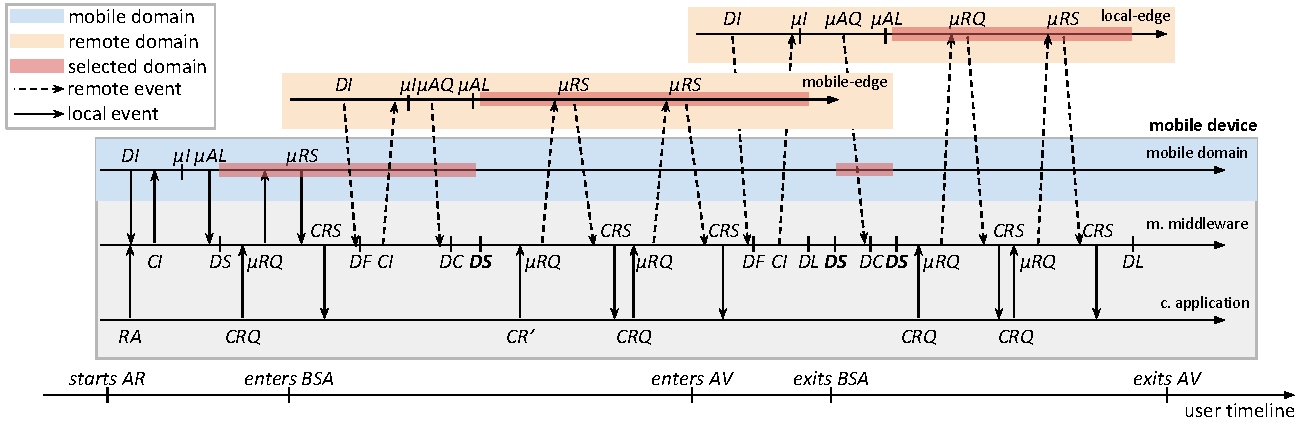
\includegraphics[width=0.95\textwidth]{figs/A3-E-instance-events}
%	\setlength{\belowcaptionskip}{-10pt}
	\caption{A timeline of events from the Running Example scenario (Sec.~\ref{sub:example}). Labels: \textit{domain identification} ($DI$); \textit{$\mu$-service identified} ($\mu I$); \textit{$\mu$-service acquired} ($\mu AQ$); \textit{$\mu$-service allocated} ($\mu AL$); \textit{domain changed} ($DC$); \textit{C-request arrived} ($CR$'); \textit{$\mu$-service request} ($\mu R$'); textit{$\mu$-service identified} ($\mu R$'') \textit{C-request served} ($CR$''); \textit{domain lost} ($DL$).}
	\label{fig:A3-E-instance-events}
\end{figure}

Figure~\ref{fig:A3-E-instance-events} depicts a timeline of events from our Running Example scenario. The timeline starts with our user initializing the AR after entering the touristic area. The mobile middleware starts with the application and receives a \textit{domain identification} ($DI$) from its mobile domain, to be replied with a \textit{client identification} ($CI$). Following the $\mu$-service identification ($\mu I$), the middleware triggers a \textit{$\mu$-service allocated} ($\mu AL$) once the corresponding functions have been registered. After selecting this domain, the middleware triggers a \textit{domain changed} ($DC$), which allows subsequent \textit{C-request} ($CR$'') events to be handled locally. As our user's device enters a base station area (BSA) featuring a mobile-edge domain, the middleware receives a \textit{domain identification} ($DI$) and repeats the previous handshake procedure. To prevent battery drain, the self-management loop decides for the mobile-edge, triggering a $DC$ once the $\mu AL$ signal arrives. After a long period of engagement with that domain, our user enters the AV featuring a local-edge domain. As this is a first contact with the AR, this domain goes through Acquisition, whose completion is indicated by a \textit{$\mu$-service acquired} ($\mu AQ$). Due to a change of network, the connection with the mobile-edge is lost ($DL$). Preventing service interruption, the middleware momentarily switches back to its mobile domain until a $\mu AL$ signal arrives from the local-edge. Upon a \textit{domain confirmed} event (omitted), it switches domain ($DC$). 

%
%The mobile middleware deals with the following events:
%
%{\small
%	\begin{itemize}[noitemsep,topsep=4pt]
%		
%		\item \textbf{C-Request arrived:} indicates the client application has sent a new request to a continuum $\mu$-service. The event contains the target $\mu$-service reference along with any parameters. The middleware must handle it by invoking the $\mu$-service from the currently selected domain.
%		
%		\item \textbf{Request served:} indicates the arrival of a response from a domain for an invoked service. The middleware must handle it with the triggering of a \textit{C-Request served} event to be handled by the client application.
%		
%		%\item \textbf{C-Request served:} indicates a given C-request has been processed. It contains the original $\mu$-service reference along with any return value(s). The client application is responsible for handling the event.	
%		
%		\item \textbf{Domain changed:} indicates a domain have been selected for a specific $\mu$-service. The middleware must handle it by resuming the invocation of any queued and subsequent C-requests to that domain.
%		
%		\item \textbf{Domain absent:} indicates no domain is available for that specific $\mu$-service. The middleware must react by queuing subsequent C-requests and, in case of latency violation, firing a \textit{C-request failed} event.
%		
%	\end{itemize}
%}%

%TODO [Danilo] requirements must be passed by the application before, otherwise the domain selection would need to happen after the request has been fired
%It also contains continuum requirements that must be taken into account by the middleware in the decision of which 

%Two types of event dictate the end of an engagement: i) the client makes no further requests after a time interval; ii) the client selects another domain; and iii) the domain manager requires the deallocation of the service instance. 

%In all three cases, resources become available in the domain. In the latter case, the client is forced to select another domain.


%In this phase the request has already been provisioned by one or more domains and the client-side middleware (CSM) has already selected a specific domain to make the request. 

%handled and parsed by the client-side middleware (CSM), and . 


%Also, one or more domains must have setup and allocated the requested service for execution and the CSM must have selected a specific domain among all providing the same service. Finally, client's request are sent, processed, received, and returned to the application.

%Current FaaS providers allow functions to be exposed as REST services. The same applies to open source platforms implementing the FaaS model. Finally, different approaches may be used to expose local computation as services in mobile platforms like Android and iOS.

%As an exception, computation provided by mobile devices can be accessed by means of local calls to functions executed by the mobile platform.

%%What: how different policies may be employed by domains and clients throughout A3-E-Process
\subsection{A3-E Process: Domain Policies}\label{sec:A3-E-policies}

\begin{figure}[tbp]
	\raggedright
	\subfloat[Different states of a given edge domain with respect to a given client application; the transitions between states triggered by domain events are guarded by policies that may vary according to the type of domain and the SLA with different applications\label{fig:A3-E-domain}] {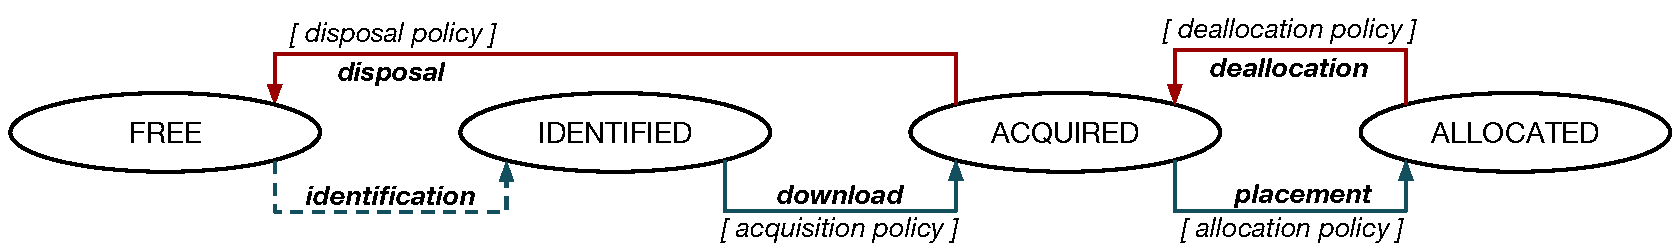
\includegraphics[width=0.95\textwidth]{figs/A3-E-domain}}\hfill
	
	\subfloat[Different states of a given client with respect to a given edge domain; the transitions between states triggered by client events are guarded by policies that may vary according to the client requirements\label{fig:A3-E-client}] {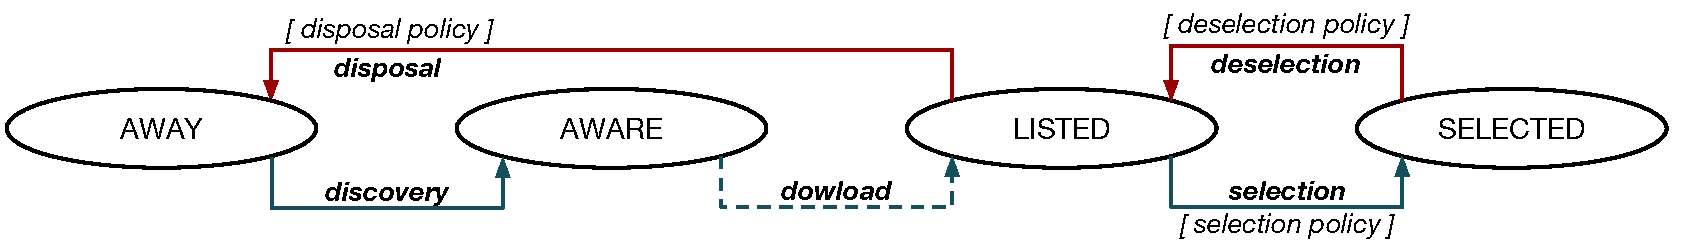
\includegraphics[width=0.95\textwidth]{figs/A3-E-client}}\hfill
	\caption{States and transitions among A3-E phases} \label{fig:A3-E-states}
\end{figure}


%What: the flexibility of A3-E model in terms of policies that regulate the transition among phases

The A3-E process is also flexible with respect to the transitions among subsequent phases. In particular, distinct policies may define different behaviors for the transition. Figures~\ref{fig:A3-E-domain} and~\ref{fig:A3-E-client} depict, respectively, the possible transitions among states of a domain with respect to a client application and vice-versa. Each state is mapped to the corresponding phase in Fig.~\ref{fig:A3-E-model}. 

From the domain perspective, policies affect the following conflicting properties: a) the \textit{efficiency} of domain resource usage; and b) the service setup \textit{delay}. Considering the first request arrival ($FRA$) from a client application as the reference event, the more \textit{reactive} the policies are to that event, the less time domain resources are likely to remain idle before it happens (more efficiency). In contrast, the chances of underutilization and idleness are higher with \textit{proactive} policies (less efficiency). Eq.~\ref{eq:setup_cost} models the total delay of service setup:

\begin{equation}\label{eq:setup_cost}
C_{SETUP} = C_{OFFLINE} + C_{RUNTIME}
\end{equation}

\noindent
in which the first term ($C_{OFFLINE}$) represents the resources required for downloading and installing the services (e.g., network and storage), whilst the later ($C_{RUNTIME}$) represents the resources needed for executing the services (e.g., memory and CPU). 

From the delay point of view, the relation is the opposite: the more \textit{reactive} the policies are with respect to the first request arrival event, the higher the delay the first request to each service is served with. In the other direction, the more \textit{pro-actively} services are made ready for execution, the lower the delay the first request to each of these services is served with. Eq.~\ref{eq:setup_delay} models the total delay of service setup:

%\Delta_{NET} + 
\begin{equation}\label{eq:setup_delay}
L_{SETUP} = \Delta_{AW} + \Delta_{AQ} + \Delta_{AL}
\end{equation}

\noindent
in which the first term ($\Delta_{AW}$) represents the time it takes for clients and domains to become aware of each other. The second term ($\Delta_{AQ}$) represents the time for acquiring all assets of a specific service, whilst the last term ($\Delta_{AL}$) represents the time for allocating resources for the service execution. 

For instance, existing cloud-based FaaS platforms (e.g., Amazon Lambda, Google Cloud Functions, and Apache OpenWhisk) employ on demand allocation of stateless functions, i.e., functions are reactively allocated upon arrival of the first request. Depending on the policy configuration, the platform waits for an idleness interval before deallocating the function~\footnote{\url{https://read.acloud.guru/how-long-does-aws-lambda-keep-your-idle-functions-around-before-a-cold-start-bf715d3b810}}. In these cases, the improved efficiency of the platform in allocating computational resources has the drawback of a setup delay (cold start). 

The domain-side policies in Fig.~\ref{fig:A3-E-domain} can be refined into three types: \textit{proactive} (P), \textit{sequential} (S), and \textit{reactive} (R). 

\begin{itemize}

\item \textbf{Proactive}: acquisition phase starts upon external event preceding the $FR_A$ event (e.g., the prediction of service usage in the near-future). Benefits: first response delay ($FR_D$) does not include $\Delta_{AQ}$. Drawback: acquired artifacts remain idle until usage. Example: stateless functions required by body device applications during a marathon event are fetched the night before the event by mobile-edge domains located along the course. 

\item \textbf{Sequential}: the beginning of acquisition phase is dictated by the completion of the awareness phase. Benefits: service artifacts are only acquired upon detection of a potential client in the domain coverage area, minimizing the likelihood of idleness. Drawbacks: $FR_D$ may include a fraction of $\Delta_{AQ}$ if $FRA$ precedes the end of acquisition. Example: stateless functions to be consumed by a mobile multiplayer game application are acquired by an indoor-edge domain inside a passenger train upon detection of two or more clients in the train.

\item \textbf{Reactive}: acquisition phase starts upon detection of a $FRA$. Benefits: acquisition of service artifacts follows an actual demand, eliminating artifacts storage idleness. Drawbacks: $FR_D$ includes $\Delta_{AQ}$, which may be disruptive for some applications. Example: stateless functions to be consumed by a TODO 

%the notion of a reactive allocation can be extended also to the acquisition of service artifacts. Instead of having functions pre-downloaded and installed, this process could happen in reaction to the first arrival of a request. 

\end{itemize}

In turn, the allocation phase can be triggered according to the following policies:

%The \textit{allocation policies} in Fig.~\ref{fig:A3-E-domain} can be:

\begin{itemize}

\item \textbf{Proactive}: allocation phase starts upon external event preceding the arrival of the first request (e.g., the prediction of service usage in the near-future). Benefits: $FR_D$ does not include $\Delta_{AL}$. Drawback: allocated resources remain idle until $FR_A$. Example: stateless functions to be consumed by connected vehicles are pre-allocated by mobile-edge domains in specific day times.

\item \textbf{Sequential}: allocation phase starts as soon as acquisition phase finishes. Benefits: depends on the acquisition policy. Drawbacks: depends on the acquisition policy. Example: stateless functions required by a marathon application running on body devices are allocated following their acquisition by the mobile-edge domains along the course.

\item \textbf{Reactive}: allocation phase starts as soon as $FR_A$ is detected. Benefits: eliminates idleness by conditioning allocation to an actual service demand. Drawback: $FR_D$ includes $\Delta_{AL}$ (cold start). Example: stateless functions required by a mobile multiplayer game are allocated by a local-edge domain inside a train following the detection of a $FR_A$ event.

\end{itemize}

%
%\begin{itemize}
%	
%	\item \textbf{Proactive}: . Benefits: . Drawback: . Example: .
%	
%	\item \textbf{Reactive}: . Benefits: . Drawback: . Example: .
%	
%\end{itemize}
%
%
%\begin{itemize}
%	
%	\item \textbf{Proactive}: . Benefits: . Drawback: . Example: .
%	
%	\item \textbf{Reactive}: . Benefits: . Drawback: . Example: .
%	
%\end{itemize}
%
%
%\subsubsection{Client-Side Policies}
%
%Clients may also adopt different policies for the selection and deselection of domains (Fig.~\ref{fig:A3-E-client}), namely:
%
%%domains are selected based on their category (cloud, edge, local) or/and 
%
%\begin{itemize}
%	
%	\item \textit{Selection policy}
%	
%	\begin{itemize}
%		
%		\item \textbf{Proactive}: 
%		
%		\item \textbf{Reactive}: 
%		
%	\end{itemize}
%	
%	\item \textit{Deselection policy}
%	
%	\begin{itemize}
%		
%		\item \textbf{Proactive}: 
%		
%		\item \textbf{Reactive}: 
%		
%	\end{itemize}
%\end{itemize}


%
%\subsection{Reference Architecture}
%
%\begin{figure}[tbp]
%	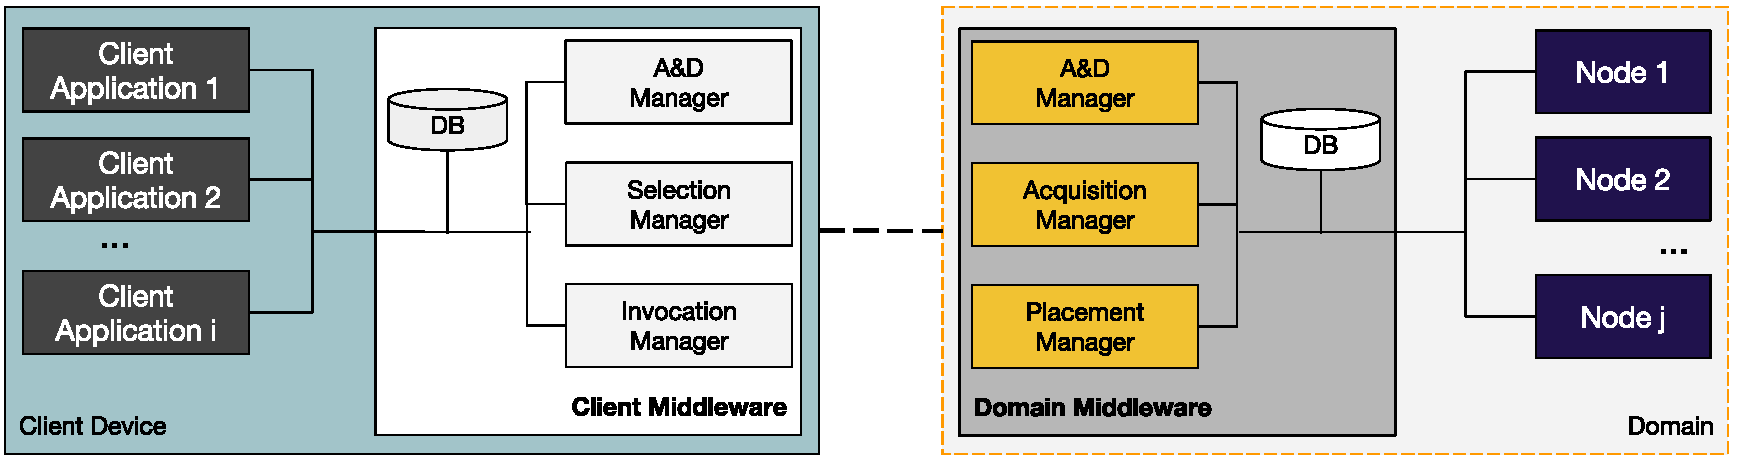
\includegraphics[width=.95\textwidth]{figs/A3-E-reference-architecture}
%	\caption{A3-E architecture in Mobile Devices and edge domains}
%	\label{fig:reference-architecture}
%	\end{figure}

	%!TEX root = ../main.tex
% -*- root: ../main.tex -*-
\section{Implementation}\label{sec:implementation}


To demonstrate the feasibility of our model
in managing the life-cycle of continuum applications, in this paper we also present working prototypes of for the domain manager and mobile middleware implementing A3-E. In particular, the former consist of a mobile domain and a local-edge domain managers, while the latter consists of a mobile middleware for Android platform devices. Later on, these prototypes are employed in the evaluation of our model.

In this paper we rely on existing FaaS platforms~\cite{AWSLambda, OpenWhisk} for handling the Allocation of $\mu$-services to a pool of dynamically allocated containers. A more sophisticated approach based on control-theory~\cite{Quatrocchi2016discrete} is considered future work (see Section~\ref{sec:conclusions} for more details).

%dedicated to the domain-side dynamic resource provisioning is considered future work;

%more precisely we will use lightweight control theoretical planners that were recently proved to be well-suited to control containerized applications~\cite{Quatrocchi2016discrete} (see Section~\ref{sec:conclusions} for more details).

%To demonstrate the feasibility of our model
%in managing the life-cycle of continuum applications
%, we describe an implementation of A3-E. Due to its complexness, in this section we focus on the self-management loops handling Allocation from both provider and client viewpoints. %Nonetheless, a complete prototype was used for the evaluation in Sec.~\ref{sec:evaluation}.

\subsubsection{Domain-side Middleware}










%Martin's old server side details

%Figure~\ref{fig:reference-architecture} shows the proposed architecture for the compute continuum. Particular focus is put on the interaction between devices and Edge domain servers, since it is the main contribution of this paper. 
%The main physical elements are mobile devices and domain servers. Mobile devices can be of any type (e.g., tablets, smartphones), running several low-latency applications that needs offloading part of their computation to more powerful servers. For this, the devices send information to be processed to the domain server through standardized network protocols~\cite{Sill17standards}.  A Base Transceiver Station\footnote{Different generations of wireless mobile networks use distinct names (e.g., eNodeB in 4G).} (BTS) bridges mobile devices and domain servers as a part of the cellular infrastructure and  Edge architecture, according to its current specifications~\cite{hu2015mobile}. In this scenario, mobile devices and Edge domain servers are at no more than a few hops from each other. These servers host a serverless infrastructure, where stateless functions are deployed and executed according to the phases defined by the A3-E model. 
%The following sections provide details about the A3-E middleware (Section~\ref{subsec:A3-E}) and the serverless infrastructure that materializes Edge domain servers (Section~\ref{subsec:ServerlessArchCont}).
%
%\subsection{Edge-FaaS}
%\label{subsec:ServerlessArchCont}
%
%Following we briefly describe the serverless architecture that materializes the notion of Edge domains --- as shown in Figure~\ref{fig:domain-edge-arch}. 
%
%\begin{figure}[htb]
%	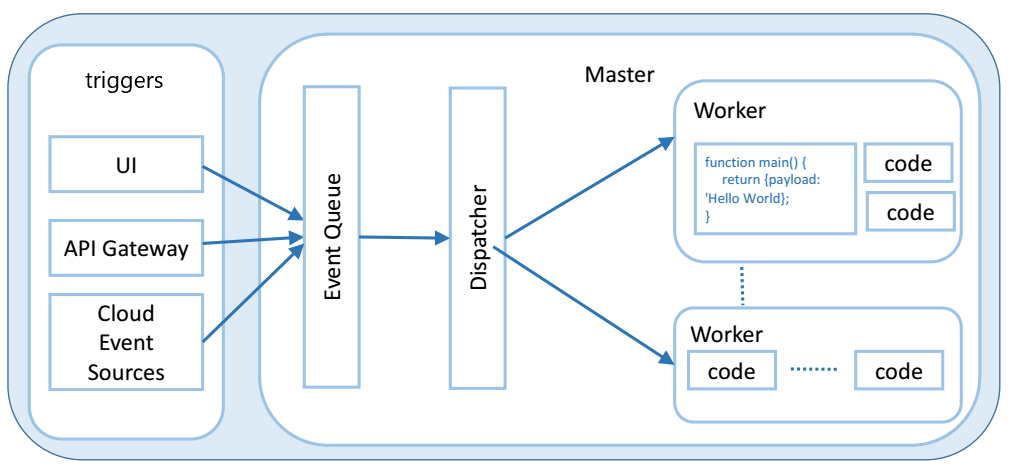
\includegraphics[width=.7\textwidth]{figs/ServerlessGenericArchEdit}
%	\caption{Serverless Architecture in the Domain Server}
%	\label{fig:domain-edge-arch}
%\end{figure}
%
%While Edge servers are ideal candidates for offloading the computation to preserve devices' battery life and reduce latency, these domain nodes are themselves potentially resource-constrained. Accordingly, the feasibility of hosting dedicated \textit{virtual machines}, \textit{containers}, and \textit{stateful applications} would also be limited, as these nodes cannot scale ``infinitely" to host always-running VMs/containers as the cloud itself. To overcome this limitation, we propose to materialize Edge domain servers through a serverless architecture~\cite{Roberts:2016,GarrigaMendonca2017}. 
%
%Figure~\ref{fig:domain-edge-arch} details the serverless components deployed on the domain server. The entry points are the \textit{triggers} associated with events --- e.g.,  mobile sensor readings or HTTP requests from mobile apps.  
%%in the MAR application, an event that triggers a function consists of uploading of an image or capturing a frame with the device's camera. --e.g., changes to database records, mobile sensor readings, code commits to a repository, or simple HTTP requests from Web or mobile apps. 
%These triggers fire requests to an \textit{Http Server} that exposes available functions as REST endpoints. 
%
%To achieve network transparency, a local Domain Name Server (DNS), deployed on the cellular infrastructure, must distinguish between requests addressed to the A3-E middleware/RESTful functions exposed by the domain server, and any other request for an Internet endpoint. The main difference from a regular DNS is locality, as the requests must be handled by the domain server on the current base station. To this end, the names of edge resources must be resolved locally without being propagated to public DNS servers. Whereas the specific details of the naming solution are outside the scope of this work, we argue that such a feature should not pose a significant technical challenge.% as it is already partially supported by the cellular infrastructure [CITE? is it right?].
%
%Once a request reaches the domain server, it is then forwarded to a \textit{controller} component, which identifies and retrieves the function being called, authorizes the execution of such a function and identifies an available invoker to run it. \textit{Invokers} isolate the \textit{functions} in containerized environments, optimized and managed by the serverless provider to reduce overhead and response time. Note that cold starts can happen when the controller allocates an inactive/new function for the first time. It increases time for the first call while the provider provisions the invoker (runtime container) and then runs the function. However, when the function is still allocated or warm --- since it was engaged recently by the same or a different client --- the environment stays alive, ready and waiting for execution. Eventually, after a period of inactivity (that depends on the size of the function and the current load of the server), the provider can drop the container and the function be deallocated, freeing resources for other functions.
%
%
%Finally, after execution, results and logging information are stored in the \textit{Storage} component, a highly available, noSQL database. Note that most of the components of the serverless architecture of the domain server are shared 
%%(in grey in Figure~\ref{fig:abstract_architecture}) 
%among all the functions. The highly shared nature and the automated management of the whole platform allows any function allocated on the domain servers to scale up automatically and elastically to unexpected bursts in the workload, and to scale down when it is not used anymore. In contrast with container-based stateful applications, the serverless platform is responsible for allocating functions of one or more applications on a pool of shared containers, according to the resources available at the domain server. As a result, the use of the computational resources of domain servers is optimized, allowing both more functions to be deployed and more requests to be processed simultaneously.
%
%Needless to say, an IaaS/FaaS cloud domain can always be selected to allocate and engage functions when required --- due to unavailability/overload of edge domain servers. Their implementation is similar to those described above, although details can vary among different vendors\footnote{\url{https://github.com/apache/incubator-openwhisk/blob/master/docs/about.md}}.
%
%As an advantage over the traditional, ``serverful'' approaches, it is not necessary to pre-allocate multiple virtual machines or containers to be resilient and responsive against downtime of single instances or bursts of workload. The on-demand execution of functions provides inherent scalability and optimal utilization as the number of running functions always matches the trigger rate. Additionally, the application developer only focuses on the application code and can fully outsource the management of the execution infrastructure to the A3-E middleware. The serverless approach also provides a fine-grained \textit{pay-per-use} billing model with benefits for both application owners and telecom operators (in charge of the domain servers).

\subsection{Mobile Middleware}~\label{sec:mobile_middleware}

%\begin{figure}[tbp]
%	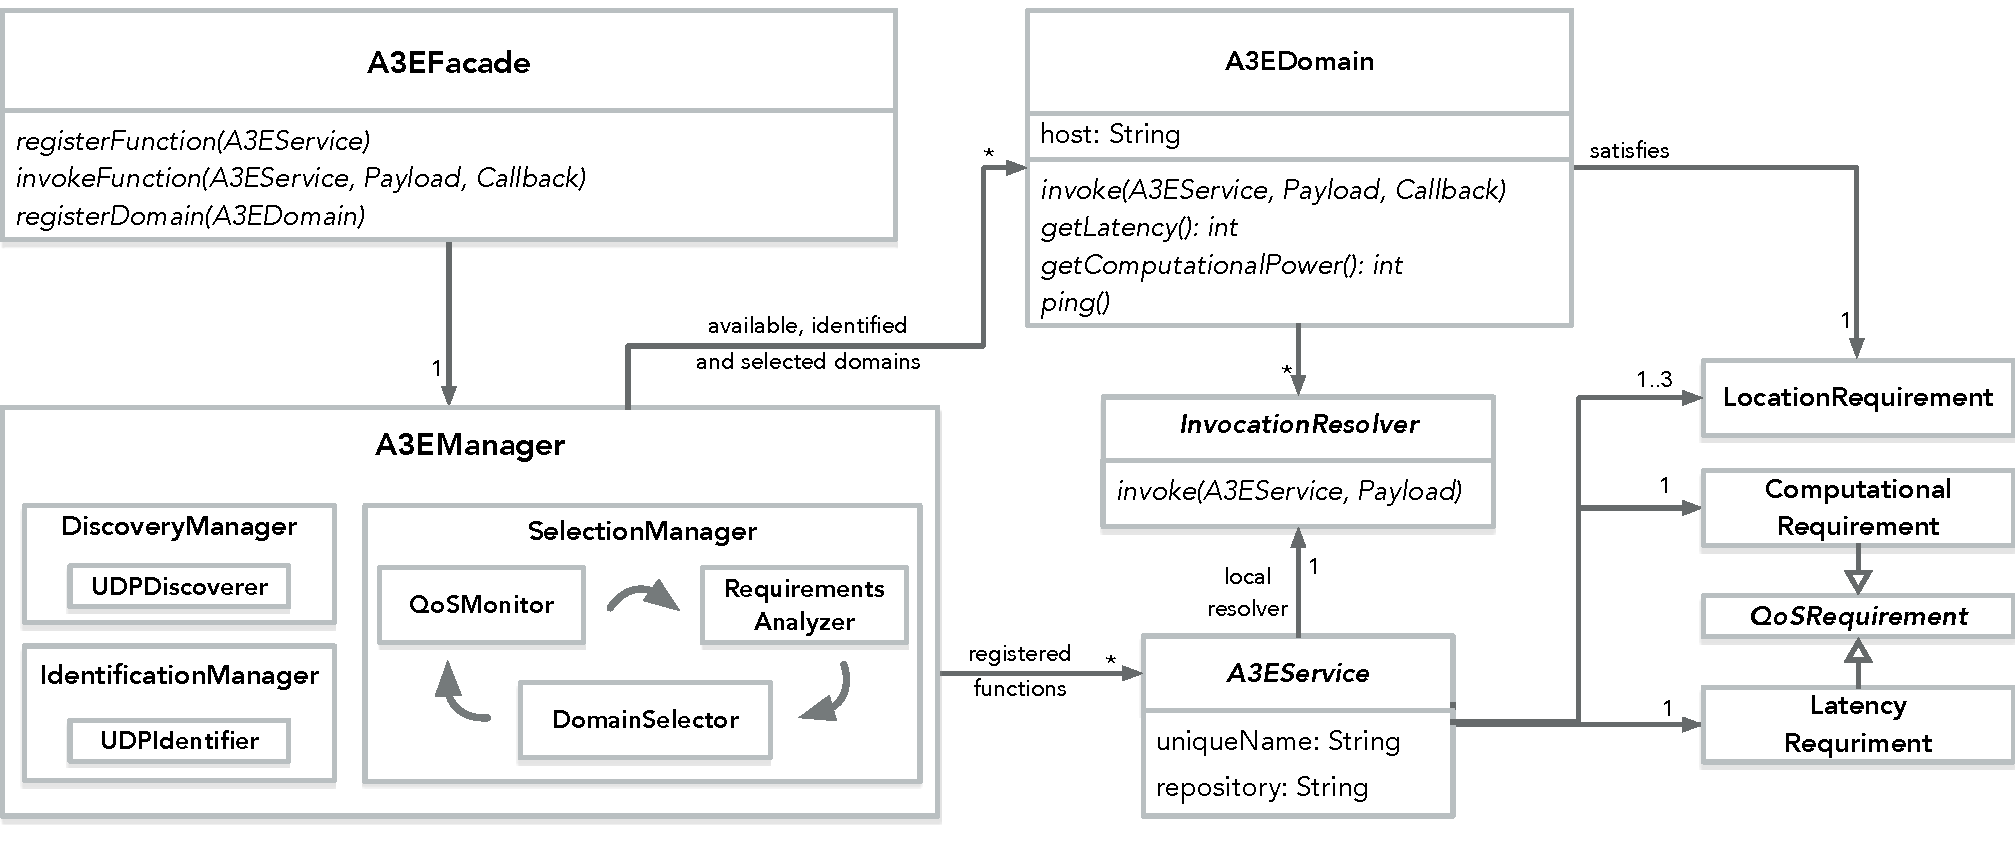
\includegraphics[width=1\textwidth]{figs/a3e-mobile-prototype}
%	\caption{Client-side Middleware Architecture}
%	\label{fig:mobile-prototype}
%\end{figure}

%TODO [Danilo] consider moving part of this nice introduction to the formulation (Sec. 2.3)
The main goal of the client-side middleware~\footnote{Documentation and source code are available at \url{https://github.com/deib-polimi/A3-E-CSM}} is to allow client applications to invoke A3-E microservices without knowing where they will actually be executed within the computing continuum: locally on the mobile domain, in a local-edge server, in a mobile-edge server, or in the cloud. Its selection algorithm is a multi-objective function that takes into account the measured QoS and the requirements. The provided implementation targets Android-based devices. However, it does not use Android-specific technology and can therefore be generalized to other mobile platforms. 

To implement Awareness, the middleware listens for \textit{domain identification} signals sent by its mobile domain and broadcasted by edge domains. To avoid battery drain, edge domains discovery happens for a short period after the mobile middleware is first executed or the device's network state changes (e.g., from a local-area Wi-Fi to a cellular network). 

For every domain found, the middleware proceeds with Acquisition by sending a \textit{client identification} signal containing a Git repository from which $\mu$-service function(s) and dependencies can be downloaded, in case of edge domains; or the qualified name of function(s), in case of the mobile domain. Finally, as in this paper cloud domains have been evaluated with an existing FaaS platform lacking A3-E's Awareness and Acquisition, cloud domains are acquired programmatically.


%Further optimization could be achieved by employing state-of-art advertisement and discovery approaches. 

The mobile middleware implements A3-E's Allocation as a self-managing loop that: (i) monitors $\mu$-services provided by different domains in terms of QoS metrics; (ii) analyzes the best alternative satisfying requirements of the client application; and (iii) updates the domain selection for a given $\mu$-service. In specific, the analysis consists of a multi-attribute rating that takes into account the measured QoS attributes and application requirements.

%TODO [Danilo] make sure we introduce requirements before or add the missing bullet below 
%In addition to A3-E's \textit{Location requirements}, 
The prototype considered three types of $\mu$-service requirements: a \textit{Location Requirement} constrains where the $\mu$-service can be placed within the continuum, i.e., \textit{LOCAL}, \textit{LOCAL\_EDGE}, \textit{MOBILE\_EDGE}, or \textit{CLOUD} or a combination of the above;  a \textit{Latency Requirement} constrains network latency, i.e., \textit{ANY}, \textit{LOW} or \textit{VERY\_LOW}; and a \textit{Computational Requirement} defines how relevant it is for a $\mu$-servi to have fast computing, i.e., \textit{ANY}, \textit{FAST} or \textit{VERY\_ FAST}. 

%{\small
%\begin{enumerate}
%	
%	\item a \textit{Location Requirement} constrain where the $\mu$-service can be placed within the continuum, i.e., \textit{LOCAL}, \textit{LOCAL\_EDGE}, \textit{MOBILE\_EDGE}, or \textit{CLOUD} or a combination of the above; 
%	
%	\item a \textit{Latency Requirement} constrains network latency, i.e., \textit{ANY}, \textit{LOW} or \textit{VERY\_LOW}; and 
%	
%	\item a \textit{Computational Requirement} defines how relevant it is for a $\mu$-servi to have fast computing, i.e., \textit{ANY}, \textit{FAST} or \textit{VERY\_ FAST}. 
%\end{enumerate}
%}%

Computational requirements defined as a fixed score ranging from $1$ to $5$\footnote{Labeling computational power is also common in the cloud where different tiers of virtual machines are available -- \url{https://aws.amazon.com/ec2/instance-types/}}. By default, the mobile domain has a score of $1$, edge domains have a score of $4$, while cloud domains have a score of $5$. As cloud provides the illusion of infinite scalability it gets the maximum score, regardless of the VMs that are actually being used. 

%with dynamic scores taking into account the saturation of the domain or the device's battery level (in the case of a mobile domain).
\setlength{\textfloatsep}{5pt}% Remove \textfloatsep
{\scriptsize
\begin{algorithm}[h]
	\caption{A3E Selection Algorithm}
	\label{alg:selection}
	\begin{algorithmic}[1]		
		\Function{selectDomain}{A3EService service, A3EDomain[] $identifiedDomains$}
		\State$scoreRange \gets 5$
		\State $maxLatency \gets \Call{computeMaximumLatency}{identifiedDomains}$
		\State $maxCpuPower \gets \Call{computeMaximumComputationalPower}{identifiedDomains}$
		\State $latencyWeight \gets service.getLatencyRequirement()$ 
		\State $cpuPowerWeight \gets service.getComputationalPowerRequirement()$ 
		\State $maxScore \gets 0$
		\State $selectedDomain \gets null$
		\ForAll{$domain \in identifiedDomains$ } 
		\State $latency \gets domain.getLatency()$ 
		\State $cpuPower \gets service.getComputationalPower()$ 
		\State $latencyScore \gets latencyWeight*((scoreRange-1)*(1 - latency/maxLatency)+1)$ 
		\State $cpuPowerScore \gets cpuPowerWeight*(scoreRange*(cpuPower/maxCpuPower))$
		\State $score \gets (latencyScore + cpuPowerScore) / (latencyWeight + cpuPowerWeight)$
		\If{$score \geq maxScore$} 
		\State $maxScore \gets score$
		\State $selectedDomain \gets domain$
		\EndIf
		\EndFor 
		\State \Return $selectedDomain$
		\EndFunction
	\end{algorithmic}
\end{algorithm}
}%

%TODO [Danilo] improve this paragraph
Algorithm~\ref{alg:selection} describes the procedure employed in the $\mu$-service selection. The algorithm computes a score ranging from $0$ to $5$ (line $2$). First, it retrieves the maximum computational power and network latency from available domains (line $3$ and $4$). Then, it retrieves the weights assigned to each QoS metric (lines $5$ and $6$). These weights correspond to the values associated to the \textit{LatencyRequirement} and \textit{ComputationalRequirement} of the $\mu$-service. The \textit{ANY} value corresponds to a weight of $0$, a latency requirement of \textit{LOW} and a computational power requirement of \textit{FAST} correspond to a weight equal to $1$, while a latency requirement of \textit{VERY\_LOW} and a computational power requirement of \textit{VERY\_FAST} correspond to a weight equal to $2$. 

For each domain, the algorithm computes the overall score (line $9$ to $14$). The latency score is computed by normalizing the value retrieved at line $10$ with the maximum latency previously computed. The normalized value ranges from $0$ to $1$, the higher this value is the higher the latency. Since a higher score should mean lower latencies, the algorithm computes the complement of this value and adds $1$ to avoid scores equal to $0$. The latency score is computed to be between $1$ and $5$, and multiplied by the $\mu$-service's latency weight (line $12$). The computational power score is computed by normalizing the domain computational power retrieved at line $11$ with the maximum value across the identified domains. Again, the score for this metric is computed to be between $1$ to $5$ and multiplied by its weight (line $13$). Finally, the overall score is the weighted average between the scores obtained by the domains for the two QoS metrics.

%Two considerations must be added for this algorithm. First, 
Algorithm~\ref{alg:selection}~\ref{alg:selection} is an instantiation of SMART~\cite{Olson1996}, in which multiple competing QoS attributes are taken into account using the following formula:
{\small
\begin{equation}
Smart(p) = \frac{\sum_{u=1}^{U} actual_{u}(p)*weight_u}{\sum_{u=1}^{U}weight_u} \label{eq:smart}
\end{equation}
}%

\noindent
where $p$ is a domain, the considered QoS attributes are network latency and the computational processing time (thus $U = 2$), and their weights are represented by the aforementioned latency and computation requirements. Note that, when available, edge domains have the highest chances of being selected, since they usually combine a low network latency and a medium-to-high computational power. 

%Accordingly, each $\mu$-service is mapped to the domain that best satisfies its requirements.

%Last but not least, during the \textit{Engagement} phase the CSM handles C-requests triggered by the client application for a specific $\mu$-service in the continuum and invokes the domain previously selected. Domains are bound to an invocation resolver: edge and cloud domains resolvers fire an HTTP request, while the resolver bound to a mobile domain will broadcast an Android event containing the request along with a callback. In particular, this broadcast is handled by the mobile domain manager.
	\section{Experimental Evaluation}\label{sec:evaluation}

\subsection{Domains Setup}

%\subsubsection{Domains}

\begin{table}
	\caption{Continuum Setup for the Experimental Evaluation}
	\label{tab:domain-exp-config}
	\begin{tabular*}{1\textwidth}{@{\extracolsep{\fill}}>{\raggedright}p{1.5cm}>{\raggedright}p{6cm}>{\raggedright}p{6cm}}
		\toprule 
		Domain & Machine Resources & Execution Environment\tabularnewline
		\midrule
		\midrule 
		Edge-Local & ubuntu/trusty64-2, 4x vCPUs, 4Gb RAM & Openwhisk, 256 Mb/Action, Python 2.7 + OpenCV \tabularnewline
		\midrule 
		Edge-Mobile & ubuntu/trusty64-2, 8x vCPUs, 16Gb RAM & Openwhisk, 256 Mb/Action, Python 2.7 + OpenCV \tabularnewline
		\midrule 
		Cloud-FaaS & N/A & AWS Lambda, 256 Mb/Function, Python 2.7 + OpenCV \tabularnewline
		\midrule 
		Cloud-IaaS & Autos Scaling Group with t2.micro instances + Amazon Linux AMI 2017  & NodeJs 6.11 server + Python 2.7 + OpenCv \tabularnewline
		\bottomrule
	\end{tabular*}
\end{table}

Table~\ref{tab:domain-exp-config} shows the different domains that were deployed to materialize the computational continuum for the experiments. Edge domains feature the Apache Openwhisk (formerly IBM Openwhisk) serverless framework\footnote{https://openwhisk.incubator.apache.org/} that manages {\em actions} (equivalent to functions). Being open-source, openwhisk is (to date) the only serverless alternative among the major vendors that can be deployed locally or on private clouds. 
%Particularly, openwhisk provides a built-in noSQL database: CouchDB, which is associated with the implemented actions through user-defined triggers and rules. 
Particularly, Edge-local domain is always placed close to the client applications/devices (one or two network hops). This deployment allows us to represent a situation where latency is close to zero, but the computational resources are highly constrained, as scaling-up is not possible due to inherent physical restrictions of the underlying infrastructure. Similarly, the Edge-mobile domain is placed on an university server, where the computational resources are less constrained, and still low latency can be achieved due to physical proximity and data locality. Note that in both cases the domains are deployed in the same LAN that originates the requests, to emulate the few-hop scenario in which devices are directly connected to their nearest Edge domains.


%In this experiment, we considered two alternatives for deploying the serverless continuum architecture, mimicking the behavior of both an edge node and a fog node (Figure~\ref{fig:exp-edge}).  

%The client application is embedded in the edge node, consisting on the postman requests and the node.js endpoint (Figure~\ref{fig:exp-setup1}). 
%On the edge-local alternative, we used a virtual machine running locally, on a regular laptop, with 4x CPU, 4x Gb of RAM and 40 Gb SSD of storage. 

%For the Fog alternative, we deployed the serverless architecture on Policloud\footnote{http://policloud.polimi.it/}, the private IaaS solution of Politecnico di Milano. Here, the computational resources are less constrained, and still low latency can be achieved due to physical proximity (two hops from the client) and data locality. This setup runs on a small cluster of 4 virtual machines with 2x CPU, 4x Gb of Ram and 100 GB SSD, each running a different component of openwhisk (triggers and storage, Http server, controller, and invokers, respectively). Note that in this case the fog node is deployed in the same LAN that originates the requests, to emulate the few-hop scenario in which devices are directly connected to their corresponding MEC.

The serverless cloud alternative (Cloud-FaaS) for this experiment uses AWS Lambda\footnote{https://aws.amazon.com/lambda/} as the first-available and most mature serverless solution in the market. The functions and associated libraries and services (storage, image recognition) are hosted in the same region, which is enforced by AWS to guarantee a certain degree of data locality. Finally, we also deployed the feature recognition functionality as a ``serverful'' Cloud setup (Cloud-IaaS). However, the main goal of this experiment is not to compare traditional cloud services against a serverless solution, but to demonstrate that the proposed continuum can outperform the Cloud under certain circumstances and requirements.


\subsection{Domain Latency Evaluation} 

In order to compare the latency along the continuum, we performed experiments with different number of parallel requests firing at a constant rate. Each request consisted on feature extraction and matching from a sample image. This experiment was performed without using the A3-E middleware, since it aims to evaluate only the different domains.

Figure~\ref{fig:exp-setup1} shows the experimental setup. Capturing and uploading an image is emulated using Postman\footnote{https://www.getpostman.com/}, a JavaScript open source application designed to load test functional behaviors and measure the performance of Web APIs. The  payload for this experiment was a sample image of approximately 65 Kb, which is a reasonable size for this use case considering the requirements regarding low-latency, computation time and battery consumption~\cite{rodriguez16mobile}. 

Then, the image is sent through HTTP/POST and different subsequent steps are executed depending on the domain: Openwhisk actions for both Edge domains, AWS Lambda functions for Cloud-FaaS domain, and a simple Nodejs server that calls a Python function for Cloud-IaaS domain.

%In our edge domains for the experiment, uploading an image to CouchDB (Step 3.a) triggers the action that performs the feature extraction and matching (Step 4.a)  with the points-of-interest, supported by the OpenCV\footnote{\url{http://opencv.org}} visual recognition library (Step 5.a). 


\begin{figure}
	
	\centering
	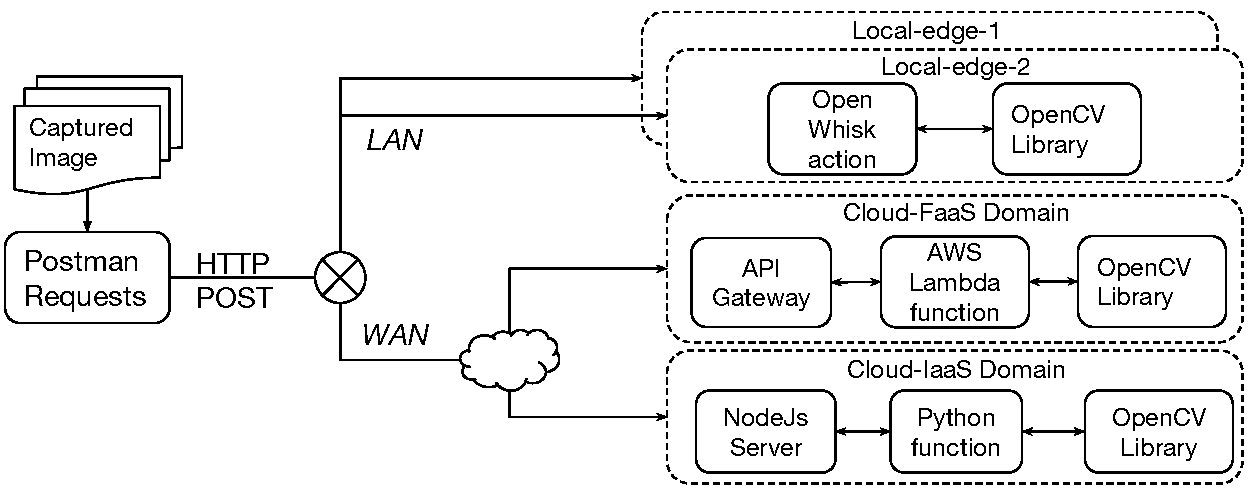
\includegraphics[width=0.9\textwidth]{figs/experimental-setup.pdf}
	\caption{Setup for Latency Experiments}
	\label{fig:exp-setup1}
\end{figure}

%\subsubsection{Baseline Latency}

To measure the latency, the workload was parameterized using different number of parallel clients, which perform 100 requests each, fired at a constant rate of two per second. This setup considers not only the default maximum for concurrent executions in AWS Lambda\footnote{http://docs.aws.amazon.com/lambda/latest/dg/concurrent-executions.html} and Openwhisk\footnote{https://github.com/apache/incubator-openwhisk/blob/master/docs/reference.md}, but also the limited resources of the edge domains. 

The experiment stresses progressively the different domains, and allows to compare the relative latency under each workload. Figure~\ref{fig:latency-domains} shows the average latency for each scenario, averaged through 5 executions. Note that the function computation time (light gray) is distinguished from the overhead (dark gray), which includes network communication (routing, forwarding) and queuing time (when no resources are available to process the request immediately). 

\begin{figure}
	
	\centering
	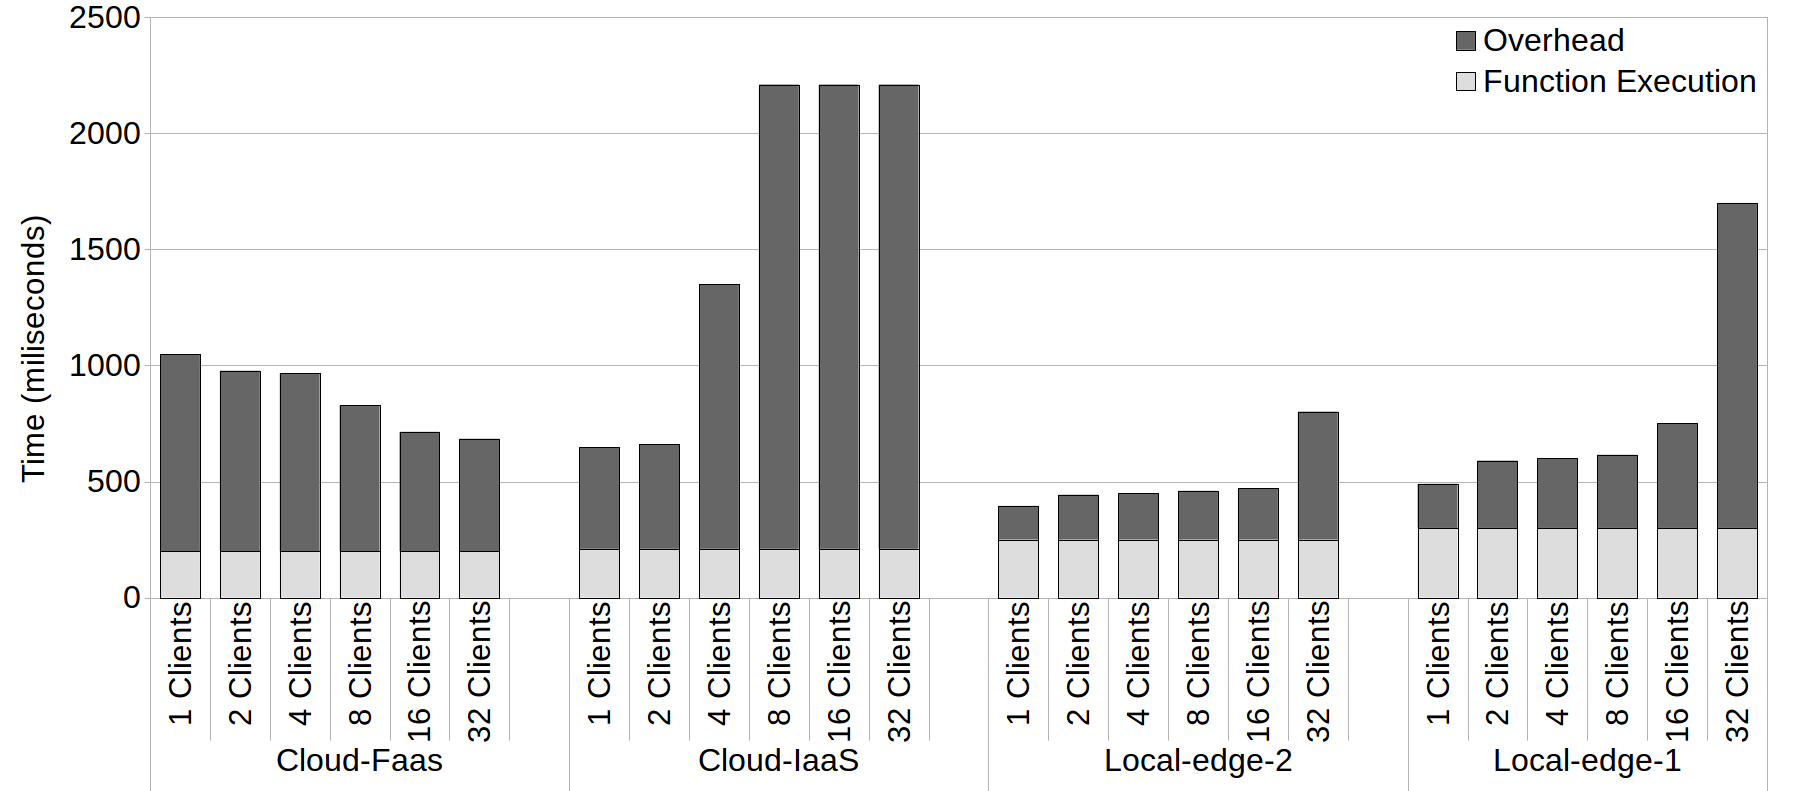
\includegraphics[width=1\textwidth]{figs/latency-domains}
	\caption{Latency results for each domain and different number of clients.}
	\label{fig:latency-domains}
\end{figure}

 For these scenarios, the latency added by the edge domains is less than the latency in both cloud alternatives, considering up to 16 simultaneous clients, with a rate of 2 $requests/second$ each. Regarding the serverless cloud alternative, the overhead reduction is up to 90\% for edge-local and up to 82\% for edge-mobile respectively. Regarding the traditional cloud domain, reductions are up to 77\% and 58\% respectively. Since a scaling-up action triggers when more than one VM instance is needed to handle the workload (that can demand several seconds~\cite{Quatrocchi2016discrete}), requests timeout in the meantime. 
 
 For light to medium workloads, the edge-local and edge-mobile domains outperformed all the other alternatives for this scenario. However, edge-local domain is the most resource-constrained, which hinders its availability under heavier workloads. Interestingly, the traditional cloud domain also outperformed the serverless one (46\% less latency) for light workloads. This can be due to the additional steps performed by the API Gateway in order to forward RESTful calls to lambda functions\footnote{http://docs.aws.amazon.com/lambda/latest/dg/with-on-demand-https.html}. Nevertheless, this advantage is mitigated by the fact that the serverless alternative is more reactive against bursts of workload, scaling faster and offering a fine-grained cost model~\cite{Villamizar2017lambda,Hendrickson:2016}.


%\subsection{Battery} The second set of experiments targeted the measurement of battery consumption of a mobile device in two scenarios: 1) in which feature extraction and matching were performed locally, and 2) these tasks were offloaded to edge servers.

\subsection{Continuum} The next set of experiments targeted the evaluation of A3-E with a computational continuum scenario. In specific, the evaluation consisted of a mobile device hosting a simplified version of an AR application with the feature extraction and matching modeled as stateless functions that can be executed locally (Java Functions), in an edge-based FaaS platform (OpenWhisk), or a cloud-based FaaS platform (Amazon Lambda). We measured the following parameters: Battery consumption, total execution time, and time per call. The experiment featured four different scenarios: With only one domain available (either locally in the device, edge-mobile or cloud-faas), and then with all domains available at the same time (all-domains). \textcolor{blue}{[TODO] (1) Explain the probabilities of having each domain available. (2) Discuss the relevance of the results} 
Figure~\ref{fig:exp-a3e} shows the results for the experiment, averaged among 5 executions for each scenario.

\begin{figure}[tbp]
	\raggedright
	\subfloat[Battery consumption (\%)\label{fig:battery-a3e}] {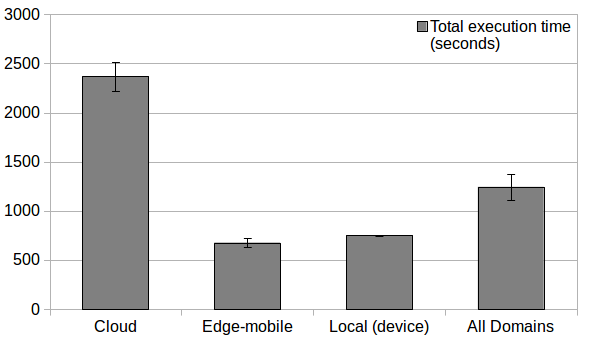
\includegraphics[width=0.5\textwidth]{figs/total-exec-time-A3E}}
	\subfloat[Total execution time (seconds)\label{fig:total-exec-a3e}] {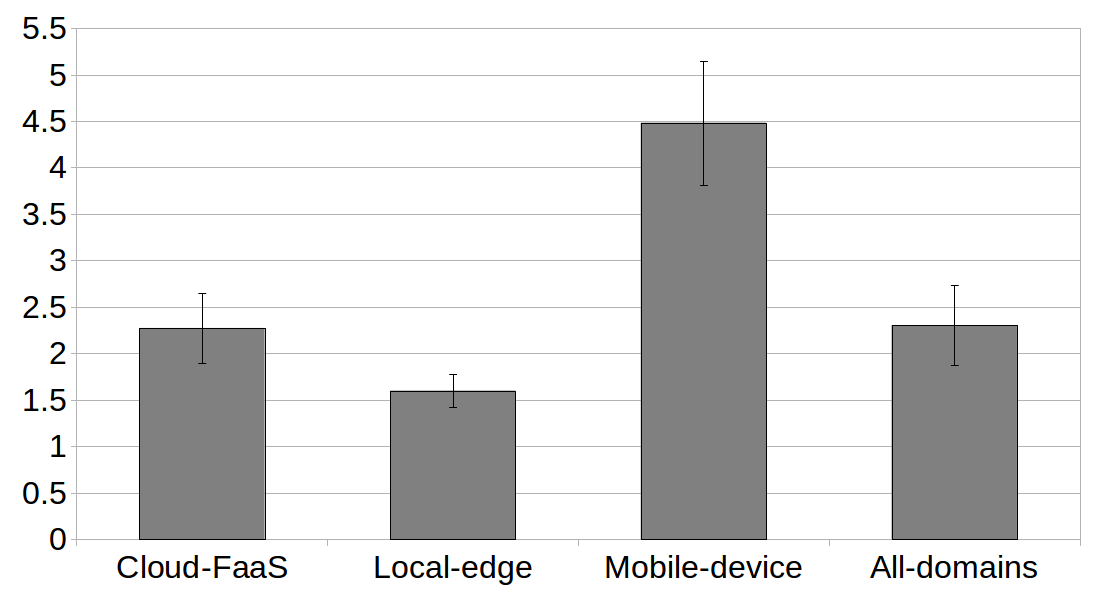
\includegraphics[width=0.5\textwidth]{figs/battery-consumption-A3E}}
	
	\centering\subfloat[Execution time per call (miliseconds)\label{fig:time-per-call-a3e}] {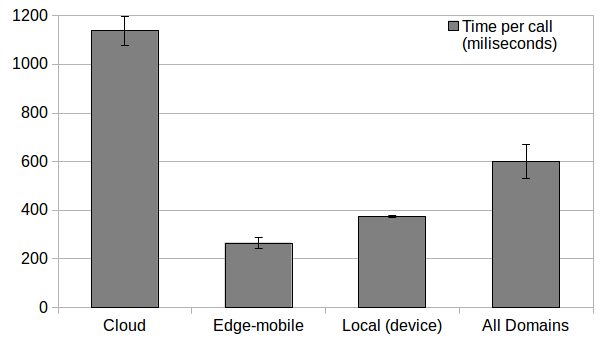
\includegraphics[width=0.5\textwidth]{figs/time-per-call-A3E}}

	\caption{A3-E experimental evaluation results} \label{fig:exp-a3e}
\end{figure}






	\section{Related Work}
\label{sec:related}

%The computational continuum
The first notion of a computing continuum was based on cloudlets (trusted, resource-rich computers or clusters of computers, connected to the Internet and available for nearby mobile devices~\cite{Satyanarayanan09cloudlets}) for a Mobile-Cloudlet-Cloud architecture capable of reducing response time~\cite{Soyata:2012}. The cloudlets are homogeneous and connected to each other to coordinate the offloading of computational intensive tasks. Static data (e.g., template images for face recognition) is stored in the cloudlets beforehand. Our approach encompasses intra-domain allocation (e.g., among cloudlets in the same domain), but also considers heterogeneous and disjoint domains among which a coordinated allocation is not feasible (e.g., among cloudlets from different providers). In the later case, allocation is performed dynamically by clients given the perceived QoS from different domains.

From a theoretical point of view,~\cite{sarkar2015assessment} compared the performance of the continuum (bridged by means of fog computing) and cloud computing in the context of IoT, showing that the continuum outperforms cloud computing as the fraction of applications demanding low-latency response increases. However, in scenarios where many applications do not have real-time response requirements, the continuum is observed to be an overhead compared to cloud-only execution.

More recently,~\cite{GuptaIfogSim17} proposed iFogSim, a toolkit for modeling and simulating resource management techniques in the continuum. It allows one to simulate the placement of different modules of real-time applications to edge devices and then measure latency, network congestion, energy consumption, and cost. Similarly,~\cite{SonmezEgdeCloudSim17} proposed EdgeCloudSim, to simulate multi-tier scenarios where multiple edge servers are running in coordination with upper layer cloud solutions, also featuring a device mobility model and a load generator. Both simulation platforms extend the well-known cloud simulator framework CloudSim~\cite{calheiros2011cloudsim}. We opted for deploying real edge domains rather than simulating them, although simulation of mobile-edge scenarios is considered as a future work.

Nowadays, realizing edge computing is seen as the novel and challenging part of the continuum. In~\cite{Nastic17ServerlessDataAnalytics}, a unified cloud and edge data analytics platform is proposed. The later extends the notion of serverless computing to the edge via a reference architecture, enabling uniform development and operation of analytics functions, hiding from the client the heterogeneity between cloud and edge. At the hearth of the model lays an orchestrator that performs a control loop. It receives the application configuration directives, in terms of high-level objectives such as optimizing network latency. It interprets and analyzes these goals and decides how to orchestrate the
underlying resources, as well as the user-defined functions, by invoking
the underlying runtime mechanisms. However, the concrete mechanisms for orchestration are left open. In contrast, the A3-E model tackles specific details regarding the autonomous self-management of FaaS-based microservices along the continuum. Additionally, this approach particularly targets data analytics applications, while our model focus on general purpose applications (particularly those with low latency requirements). Moreover, prototypes of A3-E middlewares have been implemented and evaluated. 

%This approach enables combining the benefits of the edge (lower response time and heterogeneous data management) with the computational and storage capabilities of the cloud. The proposed serverless data analytics paradigm is particularly suitable for managing different granularities of data analytics approaches bottom-up. This means that the edge focuses on local views (for example, per edge gateway), while the cloud supports global views, that is, combining and analyzing data from different edge devices, regions, or even domains. Data analytics can be performed on edge nodes, cloud nodes, or both, and delivered from any of the nodes directly to the application, based on the desired view. Moreover, the top-down control process allows decoupling of application requirements (the what) from concrete realization of those requirements (the how). This allows developers to simply define the analytics function behavior and data-processing business logic and application goals  instead of dealing with the complexity of different management, orchestration, and optimization processes.

%Computation offloading to the edge

~\cite{Satria2017mec} proposes concrete mechanisms for computation offloading among nodes located at neighbor base stations. In the context of the A3-E model, this work provides a reactive domain-side allocation scheme targeting fault-tolerance in which mobile-edge domains are modeled as the set of servers comprised in neighbor base stations. Differently from our model, this work considers mobile devices as means for relaying data from disconnected base stations. In A3-E, the disconnected computational resources are considered as different domains. However, a client-side selection is responsible for reallocating domains based on their availability and provided QoS. 

%either directly or using nearby devices as relay nodes, as a solution for overloaded edge nodes. The former is where a node offloads its work to available neighbors within transfer range, while the latter is where no neighbor nodes within transfer range are available, and uses devices as ad-hoc relay nodes in order to bridge two edge servers. In contrast, our approach mitigates the overload in the edge by first, a serverless architecture that provides an effective and efficient usage of available resources, and second by sensing the QoS in the client-side middleware to decide whether to offload the computation to the edge/cloud. Certainly, the scalability of our proposed architecture could be extended by means of a neighbor offloading strategy as proposed in~\cite{Satria2017mec}.

%In a similar direction, T\"arneberg et al.~\cite{Tarneberg2017} proposed a model that bridges mobile edge computing and the distributed cloud paradigm, as well as an algorithm to solve the resource management challenges that emerge from this integration. I or by an integration of MEC and cloud resources as proposed in ~\cite{Tarneberg2017}.

In a similar direction,~\cite{Tarneberg2017} proposes an algorithm for application placement and resource management across an heterogeneous topology comprised of cloud and edge computing. 
%This approach stresses the challenges for such an heterogeneous topology as meeting all client applications’ SLAs, minimizing infrastructure-wide operational expenditure and load balance of resources and mitigate resource usage skewness. 
The algorithm solves a multi-optimization problem considering application
execution cost and the overload penalty on each node in terms of latency, as well as edge resources in the system. The objective function is constructed from the infrastructure provider's viewpoint (i.e., Telecom operators), whose objective is to minimize the overall running cost~\cite{weber2017facilitating}. We also envision a heterogeneous continuum, though we consider autonomous and independent \textit{domains} that cannot communicate and coordinate resource allocation. The proposed placement algorithm complements A3-E, as it could be employed by providers of multiple domains to optimize their costs (e.g., by restricting the availability of resources at different mobile-edge domains in certain conditions). In turn, A3-E tackles the adaptation to the conditions imposed by providers (e.g., with the deallocating of low-priority microservices from these domains and the consequent client-side selection of alternative domains).

%be seen as a first step to decide whether to use proactive or reactive allocation for each domain and application. From then on, the availability also depends on what is perceived by the clients, thus the placement is coordinated through the middleware. 

The Enorm framework~\cite{wang2017enorm} for edge node resource management enables the use of the cloud in conjunction with edge by deploying a cloud server manager on each application server. This server communicates with potential edge nodes requesting computing services, and deploys partitioned servers on the edge node, and receives updates from the edge node to update the global view of the application server on the cloud. Each edge node maintains local data, relevant to the users on its coverage area. The global view is then maintained on the cloud and updated periodically by edge nodes. When edge nodes cannot provide computing services nor improve the QoS of the application, users connect to the cloud application server as in a typical cloud scenario. The allocation follows a hierarchical approach, with a centralized control starting from the cloud and spreading to the edge nodes. In turn, A3-E offers a decentralized approach in which autonomous clients and domains are able to coordinate the placement of computation along a mobile-edge-cloud continuum. 

%, without depending necessarily on the cloud to decide the offloading. %Although the data management aspect on Enorm can complement our approach, it does not consider 
%and can be complementary to our work by addressing data locality and replication problems at architectural level sinc
%For this reason, offloading is dynamically decided by A3-E on the client side according to the perceived QoS of the available domains. 
%\textcolor{blue}{[Gupta IfogSim]}


In industry the first real-world prototype of the mobile edge~\cite{beck2014mobile} (by Nokia Siemens and Intel~\cite{NokiaMEC13}) features base stations equipped with commodity hardware, and application deployment is based on virtualization and containerization technologies~\cite{ismail2015icos}. Applications running on the mobile edge are expected to be event-driven, which complements the A3-E model that currently relies on request/response RESTful calls. However, this approach does not take into account the inherent resource limitations of edge computing, tackled by A3-E by adhering to the FaaS execution model.
%This industry prototype suggests that end users
%benefit mostly from reduced communication delay, benefiting computation intensive applications by means of offloading (as shown throughout this paper). Meanwhile, Telecom providers benefit from bandwidth consumption reduction and better scalability, while application providers profit with respect to faster
%services.

Finally, Lambda@Edge\footnote{http://docs.aws.amazon.com/lambda/latest/dg/lambda-edge.html} is a new functionality of AWS that allows one to explicitly deploy lambda functions to certain (coarse-grained) edge locations. The functionality covered by Lambda@Edge is still limited to a few scenarios, all of them tied to CloudFront (the AWS content delivery network) events. 
%In turn, A3-E deals with heterogeneous and general purpose applications and is not tied to any particular source of events.
%, that is, when a user request to see a given content, when the request is forwarded to the cloud (because such content was not available at the edge location), and vice versa for the response.

%EdgeScale~\cite{Lara2016hierarchical}, by Huawei, also brings the notion of serverless to the edge. It implements serverless functions, storage, routing and additional capabilities from scratch (while we opted for current open technologies such as Apache Openwhisk) in a hierarchy of edge data centers, over a network between the user and traditional wide-area cloud providers. Once again, this proposal does not consider independent (and potentially disjoint) domains. Besides, EdgeScale is on an early stage and does not report any empirical evaluation of latency, throughput, bandwidth and cost.

%

%according to their CloudFront content delivery service, which consists of approximately 90 edge nodes worldwide. However,  In contrast, we consider the continuum to be fine-grained, with nearby domains distributed one every $km^2$ or less. Furthermore, the upcoming  small 5G cells and microcells~\cite{beck2014mobile} allow us to think of one local-edge domain per block, or even per building in certain vital places, such as government buildings or transport stations.








%\subsection{Edge and Mobile Edge}
%The work in~\cite{beck2014mobile} provides technical details of a real-world mobile-edge prototype platform (by Nokia and Intel), together with a taxonomy of applications that can leverage such a platform. In line with our work, mobile-edge servers on base stations are equipped with computational capabilities and application deployment is based on virtualization technologies. Applications running on the mobile edge are expected to be event-driven, as in the serverless model. Moreover, identified use cases encompass offloading and local connectivity, both aspects covered by A3-E. 

%Ismail et al.~\cite{ismail2015icos} evaluated different aspects of the deployment and operation of a container technology locally on edge nodes. In their work, a testbed was setup using a database and three edge nodes interconnected by a company network. Despite the similarity with this work, our proposal goes beyond virtualization and containerization of application logic, in favor of serverless computing to optimize the use of edge resources.

%Certainly, the scalability of our proposed architecture could be extended by means of a neighbor offloading strategy as proposed in~\cite{Satria2017mec} or by an integration of MEC and cloud resources as proposed in ~\cite{Tarneberg2017}.

%mitigates the overload in MEC servers by deploying a serverless architecture on them, which provides an effective and efficient usage of available resources.  As we envision an heterogeneous continuum in which edge nodes may not be aware of each other (e.g., a domestic edge node may not be connected with a mobile one).

%. One recovery scheme is where an overloaded MEC server offloads its work to available neighbors within transfer range. The other recovery scheme is for situations when there is no available neighboring MEC within transfer range, and uses devices as ad-hoc relay nodes in order to bridge two MEC servers. 

%\subsection{Serverless Architectures}

%IBM OpenWhisk is an open source experimental FaaS started in 2016. It provides a programming model to upload event handlers to a cloud service, and register the handlers to respond to various events or direct invocations from web/mobile apps or other endpoints.

%Google Cloud Function is another service started in 2016 and still in alpha-release. Functions can be triggered by any Google service that supports cloud  pub/sub, cloud storage, arbitrary web hooks or direct triggers.

%Microsoft Azure Functions supports integration with other Azure products, plus timers and arbitrary applications via webhooks or HTTP triggers, and on-premises via the service bus.

%Webtask.io supports scheduled tasks in addition to events, but as a stand-alone tool – those events arrive via webhooks and HTTP endpoints. Webtask.io is built atop CoreOS, Docker, etcd and fleet, with bunyan and Kafka for logging.

%Finally, OpenLambda is an academic effort towards an open-source serverless architecture~\cite{hendrickson2016serverless}, consist of a number of subsystems that coordinate to run Lambda handlers, including a local execution engine that sandboxes handlers, a load balancer, and a distributed database. 

%The idea of bringing serverless capabilities to the edge is very recent. The first documented efforts date form 2017, and come mostly from the industry. 

%\textcolor{blue}{ Gartner predicting that smartphones would be the Internet access device of choice by 2018 [25 IFOGSIM Gartner]. }  

%\textcolor{blue}{  }

%\textcolor{blue}{ Within this proposal, the \textbf{Serverless Stream Model} an extension of the traditional stream processing model. The transformation function is the core concept and encapsulates user-defined data analytics logic to process data along the stream. These functions are then composed into topologies that enable complex data processing applications.  The wrapper is responsible for encapsulating the transformation functions and exposing a thin API layer, enabling the analytics function layer to treat functions as \textbf{microservices}.  For stateful functions, these wrappers also provide implicit state management. The wrapper transparently handles state replication and migration, and access to a function’s state is controlled via the exposed API. }


%\textcolor{blue}{  ENORM framework, uses the following five components on the edge node:	Resource allocator keeps track of the available CPU cores and memory. Edge Manager is composed by the node manager (deals with the requests obtained by the server manager from a cloud server) and server manager (initializes containers, allocates ports and security). Monitor, since each application edge server is monitored periodically by tracking communication/computing latency (through pings and timestamps on server logs respectively). Auto-scaler dynamically allocates/deallocates hardware resources to the containers executing application servers. Finally, Application Edge Server is the actual server that consists on a partition of the cloud server, hosted on the edge node. } ENORM is particularly focused on resource management (top-down) from cloud to edge. We envision a bottom-up approach in which execution is firstly attempted at edge nodes and then going up in the hierarchy given the unfeasibility of running near to the devices.



	\section{Conclusions and Future Work}\label{sec:conclusions}

%Due to its particular characteristics, which inherit and complement those of serverless computing, A3-E provides a suitable model for the realization of edge computing as part of a  computational continuum composed of cloud, edge, and mobile clients.

	
	\section{Supplementary Materials}	
	
	\begin{printonly}
	  See supplementary materials for the prototype implementations in the online version.
	\end{printonly}
	
	\begin{screenonly}
	
	\subsection{DSM Prototype: Local-edge Domain}

\begin{figure}[tbp]
	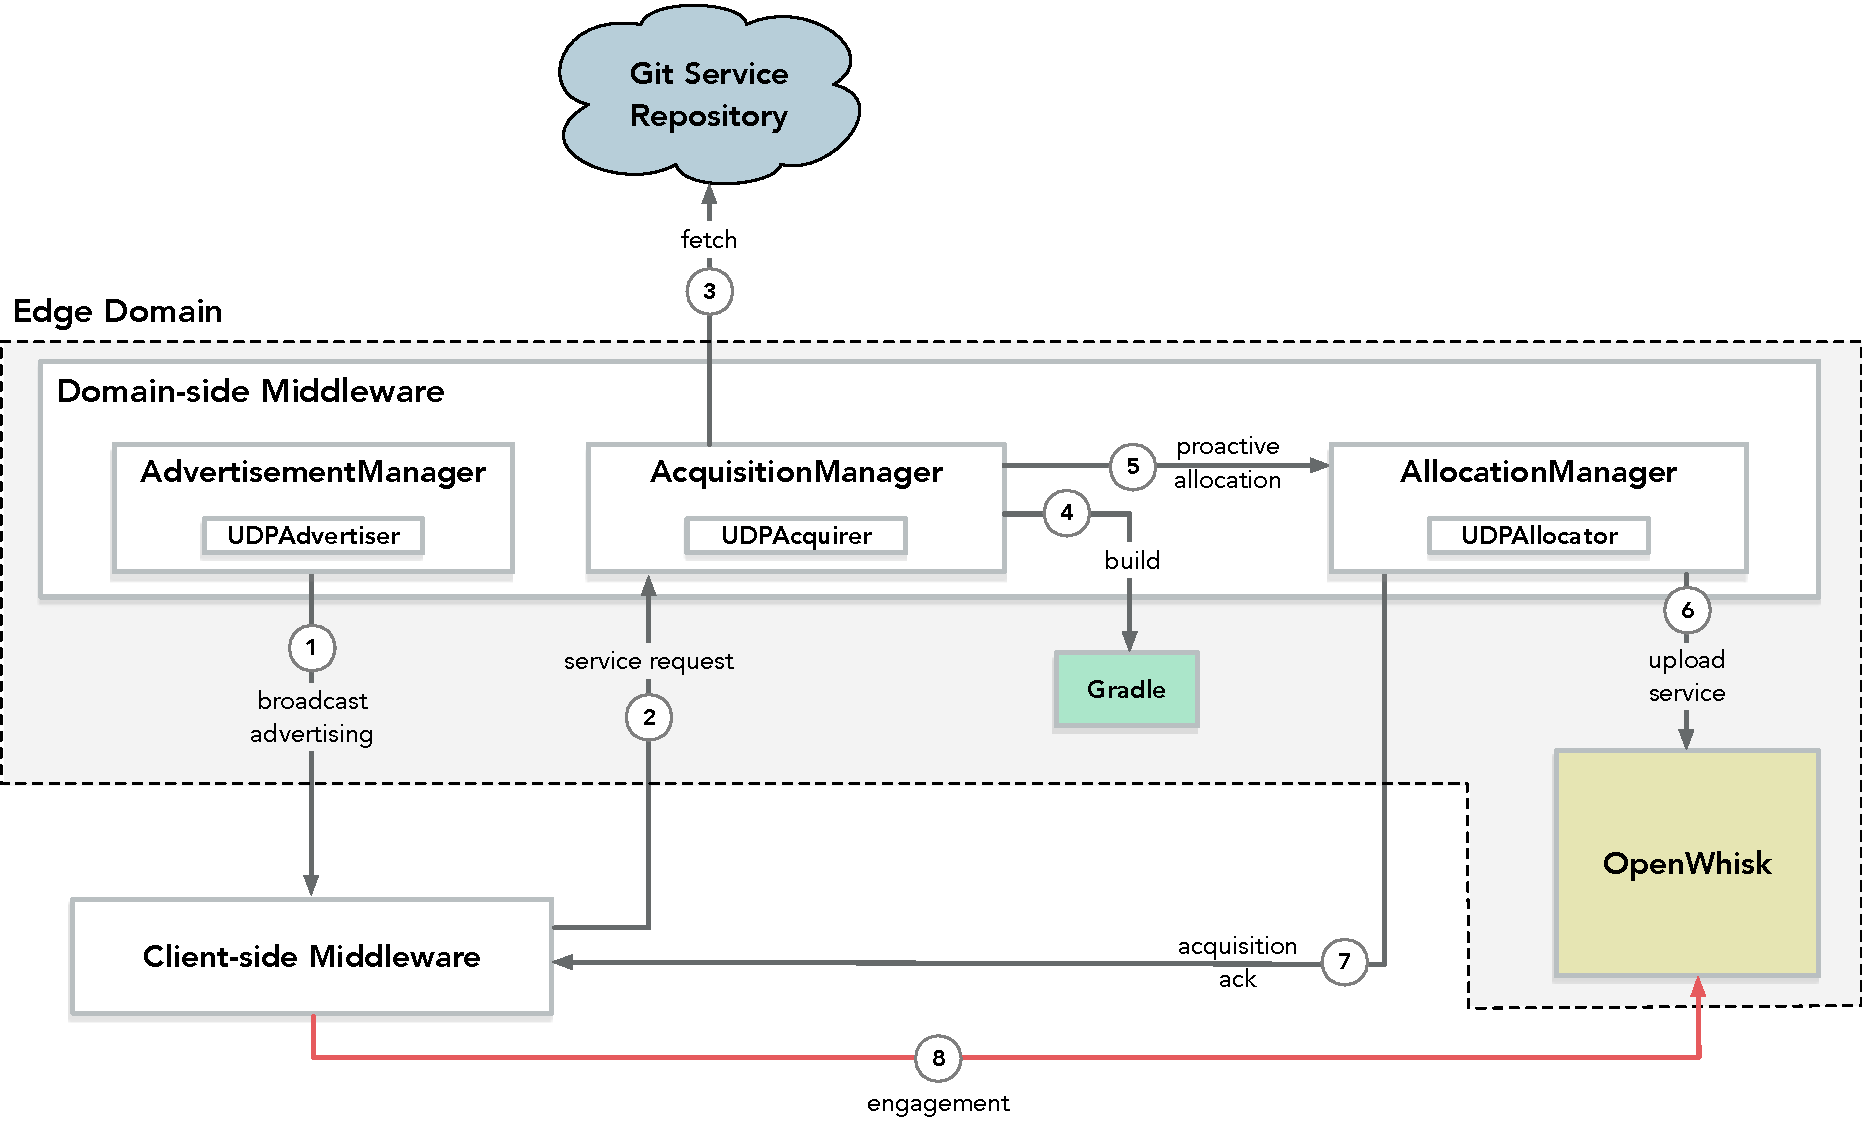
\includegraphics[width=0.9\textwidth]{figs/a3e-domain-prototype}
	\caption{Domain-side Middleware Architecture for Edge local Domain}
	\label{fig:local-edge-domain-prototype}
\end{figure}

The local-edge DSM depicted in Fig.~\ref{fig:local-edge-domain-prototype} was implemented in Python and runs within a Linux-based domain that also hosts OpenWhisk. Next, we provide a more detailed description of its implementation and behavior.

As part of the Awareness phase, an \textit{AdvertisementManager} broadcasts UDP messages (step 1) using a port that is known by the clients, with a frequency that is configurable (the default value is $5$ seconds). A unicast channel is also created through which new clients should reply (step 2) to the discovery of a domain using the address extracted from the advertisement broadcast, and a port known in advance. The CSM replies with the specification of its requested microservices (one reply per microservice) along with the public repository (e.g., Git) from which its artifacts can be downloaded.

As part of the Acquisition phase, the \textit{AcquisitionManager} downlaods (or updates existing) microservices (step 3). Among the downloaded files, a service descriptor provides information about when and how to build (step 4) source files with the microservice function(s) to be deployed to the FaaS platform. In specific, the prototype employs Gradle\footnote{\url{https://gradle.org/}} in the build process of Java functions into \textit{jar} files accepted by OpenWhisk. As an example, Listing~\ref{lst:service-descriptor} illustrates the descriptor of an image recognition service with a single Java function and two dependencies used for image classification.

Upon triggering of the Allocation phase (step 5), the \textit{AllocationManager} deploys the acquired function(s) to OpenWhisk (step 6) by means of its command-line API, and returns a message to the client-side middleware with the final endpoint of the deployed microservice along with the result of the operation (step 7). In particular, a RESTful endpoint will be created for single function in the service descriptor with the \textit{web} property assigned with value \textit{true}. From this moment on, the microservice is ready to be engaged by the client (step 8). Note that whilst the endpoint is mapped to a single function, the later may perform internal calls to other functions, effectively composing the microservice.

\definecolor{lightgrey}{gray}{0.994}
\definecolor{blue}{rgb}{0, 0, 0.25}

\lstset{
	backgroundcolor=\color{lightgrey},
	basicstyle=\footnotesize\color{black},
	string=[s]{"}{"},
	stringstyle={\footnotesize\bfseries\color{blue}},
	comment=[l]{:},
	commentstyle={\footnotesize\color{black}},
	upquote=true,
	%numbers=left,
	%numbersep=5pt,
	%numberstyle=\tiny\color{black}    
}

\begin{minipage}{.9\linewidth}
\begin{lstlisting}[caption=Image recognition service descriptor, label=lst:service-descriptor, captionpos=t]
{
 "service-name": "image-recognition",
 "functions": [{	
  "language": "Java",
   "name": "image-recognition",
   "source": "it.polimi.a3e.imagerecognition.ImageRecognition",
   "build": "true",
   "web": "true" }]
 "dependencies": ["NetSSD_deploy.prototxt", "NetSSD_deploy.caffemodel"]
}
\end{lstlisting}
\end{minipage}

\subsection{DSM Prototype: Mobile Domain}

\begin{figure}[tbp]
	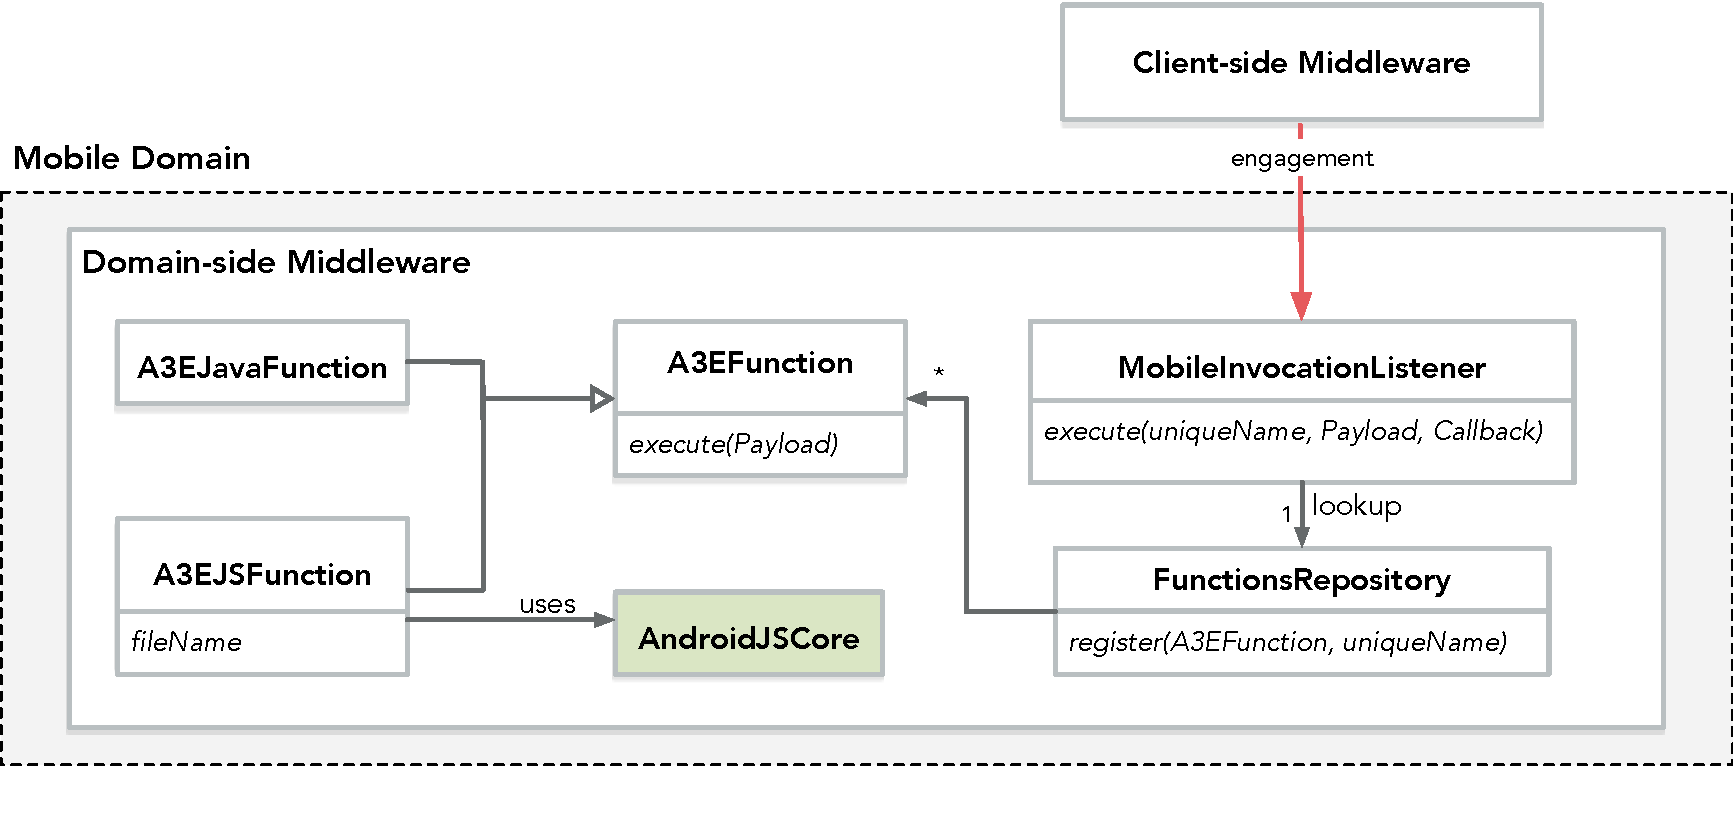
\includegraphics[width=0.9\textwidth]{figs/a3e-mobiledomain-prototype}
	\caption{Domain-side Middleware Architecture for Mobile Domain}
	\label{fig:mobile-domain-prototype}
\end{figure}

The provided mobile domain DSM prototype is depicted in Fig~\ref{fig:mobile-domain-prototype}. Next, we further detail its implementation and behavior.

%As depicted in Fig.~\ref{fig:mobile-domain-prototype}, the mobile-domain DSM implementation consists of a 
Client applications register functions to their mobile domain using component \textit{FunctionsRepository}. The prototype supports two types of functions: \textit{A3EJavaFunction} and \textit{A3EJSFunction}. In particular, \textit{A3JSFunction} represents JavaScript functions loaded from a \textit{.js} file. The latter use \textit{AndroidJSCore}~\footnote{https://github.com/ericwlange/AndroidJSCore}, an Android Java JNI wrapper required for the execution of JS code by Android applications.

The \textit{MobileInvocationListener} class handles specific Android broadcast events created by the CSM. The request is for a microservice identified by a \textit{unique name}, and is used by a \textit{FunctionsRepository} in the lookup of the corresponding \textit{A3EFunction}. For each request, the corresponding function is called with the original payload from the microservice request, which also contains a callback to be invoked as a function return.


\subsection{CSM Prototype: Android Platform}

%As described in Section~\ref{sec:proposal}, the CSM component interacts with DSM from different domains that could be either discoverable using a DNS-like mechanism or advertisement. 


\begin{figure}[tbp]
	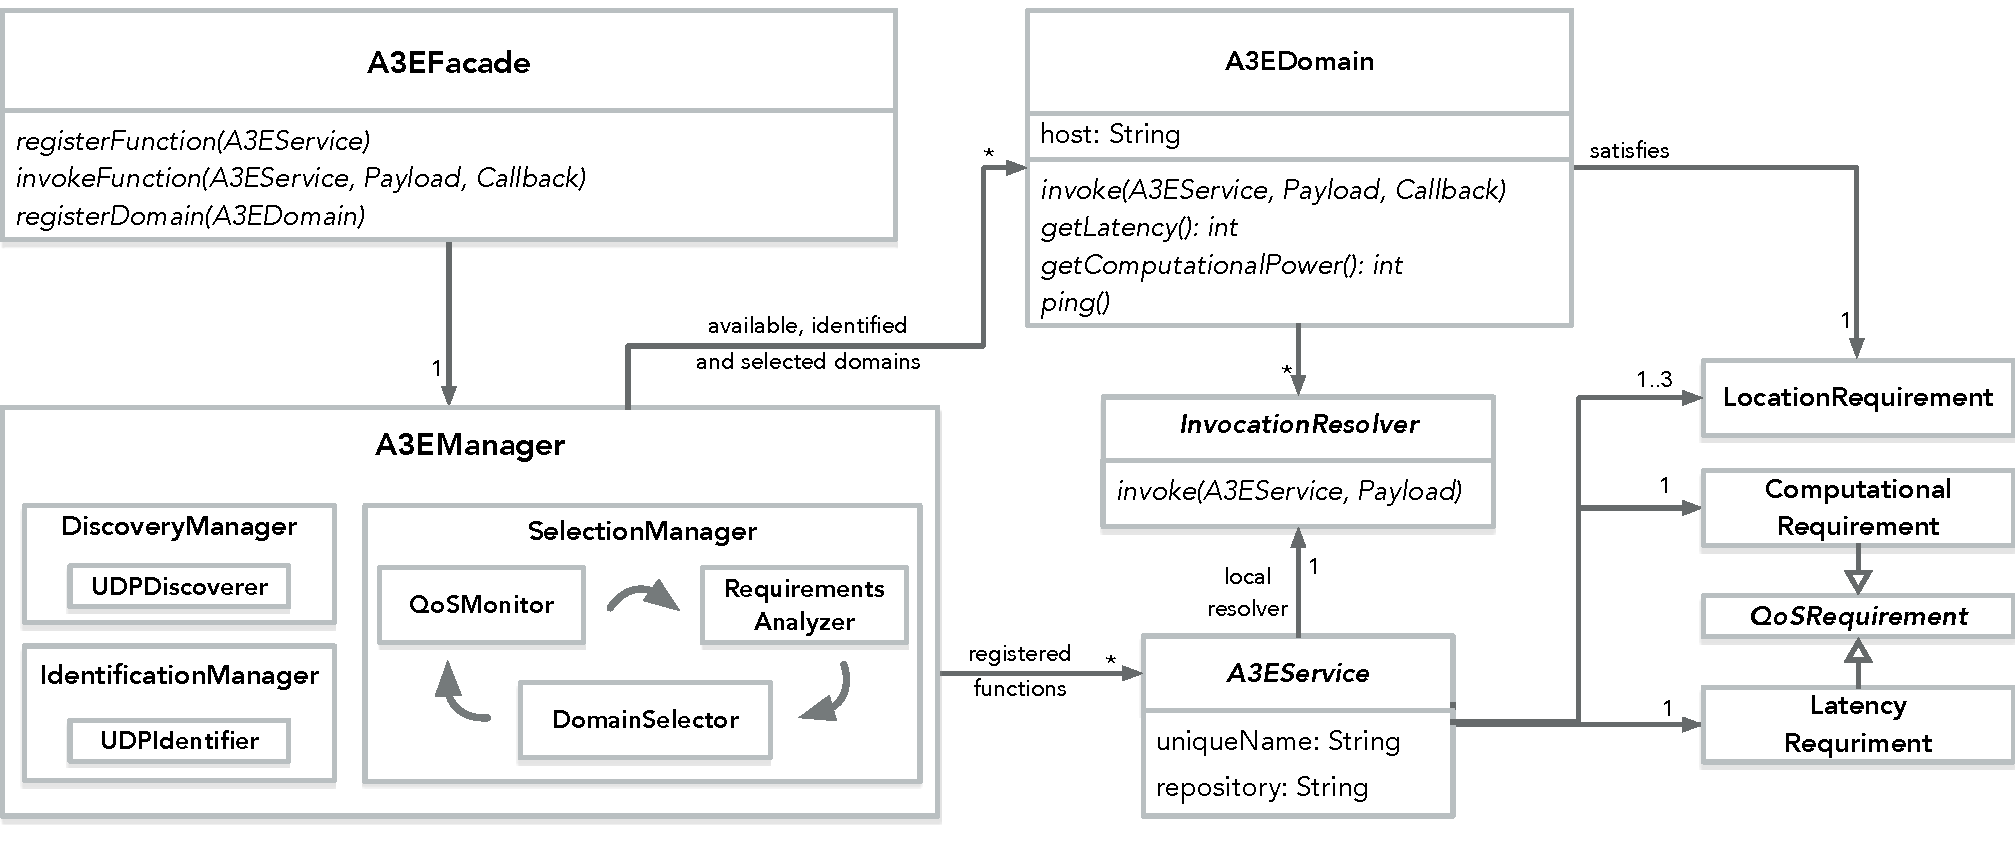
\includegraphics[width=1\textwidth]{figs/a3e-mobile-prototype}
	\caption{Client-side Middleware Architecture}
	\label{fig:mobile-prototype}
\end{figure}

Figure~\ref{fig:mobile-prototype} shows the high-level architecture of the client-side middleware. Client mobile applications interact with two components: \textit{A3EService}s and \textit{A3EFacade}. The former abstract the actual microservices to be invoked, while the latter is used to register and invoke the domain's microservices. 

An \textit{A3EService} is identified by a unique name and the url of its git code repository. It may also specify three types of requirements: 
%that corresponds to the name of the function asset that must be communicated to the continuum domains to be first acquired and then executed. Moreover each function must declare a set of non-functional QoS requirements that are organized in three types: 

\begin{enumerate}


	\item \textit{Location Requirement}s constrain where the microservice can be placed within the continuum, i.e., \textit{LOCAL}, \textit{LOCAL\_EDGE}, \textit{MOBILE\_EDGE}, or \textit{CLOUD} or a combination of the above; 


	\item a \textit{Latency Requirement} constrains network latency, i.e., \textit{ANY}, \textit{LOW} or \textit{VERY\_LOW}; and 
	

	\item a \textit{Computational Requirement} defines how relevant it is for a microservice to have fast computing, i.e., \textit{ANY}, \textit{FAST} or \textit{VERY\_ FAST}. 


\end{enumerate}

%Before becoming able for execution, the function must be registered using the \textit{A3EFacade}. 

%\begin{itemize}
	%\item \textit{Location Requirement}s are constrains over the continuum. A function can declare where it could be executed choosing a combination of three values: \textit{LOCAL}, \textit{EDGE} and \textit{CLOUD}. By default an \textit{A3EFunction} supports all three domain types but one can implement a function that, for example, cannot be executed locally thus only the \textit{EDGE} and \textit{CLOUD} requirements should be added.    
	%\item \textit{Latency Requirement} expresses how important for a function is to have a low networking latency. The default value is \textit{LOW} since the main motivation of the work is to support low-latency applications. An \textit{A3EFunction}  can  also state that this requirement should be \textit{ANY} or \textit{VERY LOW}. The lower the latency requested the more the networking latency will be considered important in the the domain selection procedure.
	%\item \textit{Computational Requirement} defines how relevant for a function is to have a fast computing processing. The predefined value is \textit{FAST}, since, again, the main targets of the approach are applications that requires fast request/response interactions. Similarly to the latency requirement two additional values are available:  \textit{ANY} or \textit{VERY FAST}. The higher  processing power is requested the more this metric will be considered important during the domain selection phase.
%\end{itemize}

%An \textit{A3EFunction} that support the \textit{LOCAL} location requirement should also define a local \textit{InvocationResolver}. As we are going to discuss later in this section, invocation resolvers deal with the invocation technology \textit{heterogenity}  of the continuum. For what regards the local domain we currently support the execution of native Java code and Javascript functions (that could be imported in the project as standard \textit{.js} files). For this purpose we created two \textit{InvocationResolver}s that can execute respectively Java or Javascript functions if the local domain is selected.

The \textit{A3EFacade} component wraps the \textit{A3EManager}, which manages all the registered \textit{A3EService}s. It consists of the discovery, identification and selection of domains, corresponding to the \textit{Awareness}, \textit{Acquisition}, and \textit{Allocation} phases of the A3-E model. 

%The loop manager consists of three main components called \textit{DiscoveryManager}, \textit{IdentificationManager} and \textit{SelectionManager}. 

Component \textit{DiscoveryManager} manages the discovery of domains. The local domain is registered when the middleware is created, while cloud domains are registered by the client application, and their endpoints must be known a-priori. Edge domains, on the other hand, are found at run time. Every time the IP address of the client device changes, the manager starts listening for UDP broadcast messages using component \textit{UDPDiscoverer}. If a message is received within a fixed timeout of $10$ seconds, the IP address of the sender is retrieved. A new \textit{A3EDomain} is then created in the middleware and added to a list of available domains. Each \textit{A3EDomain} is identified by a \textit{host} name (URI) and satisfies a specific \textit{LocationRequirement}. 

%Everytime the connection the domain is lost, the \textit{DiscoveryManager} updates its list of available domains.

 %Component \textit{InvocationResolver} is then used to actually invoke the micro-services. 

%An  \textit{A3EDomain} could be either \textit{static} or \textit{dynamic}. Static domains are added to the discovery manager at launch time, meaning that it is known a-priori that they will be available. Example of this are cloud and local domains. On contrary dynamic domains can be found only at runtime with appropriate technological protocols (such as DNS and advertising). Edge domains are not known a-priori thus they are considered dynamic. Static domains can be added by the client application using the \textit{registerDomain} operation provided by the \textit{A3EFacade} while dynamic domains are automatically discovered by the \textit{DiscoveryManager}.
 %\textit{A3EDomain}s  are identified by a \textit{host} name, that is a unique network identifier by which it is possible to interact with the domain using a network. Moreover, as shown in the figure, a domain is considered \textit{Pingable} that means that it is possible to check for its availability and measure its networking latency (in milliseconds). Each domain satisfy a \textit{LocationRequirement}, intuitively local domains satisfies the \textit{LOCAL} requirement, while the edge and cloud ones the \textit{EDGE} and \textit{CLOUD} respectively.  A domain also provides three additional operations: one to execute a function within the domain, one to retrieve the networking latency (its value is lazily updated after a \textit{ping}) and one to obtain its computational power. Finally a domain also uses an \textit{InvocationResolver} to actually invoke the function. 


%The output of this process is the list of the available domains. 
 %This component initializes the identification phase for each new available domain (e.g., domains discovered for the first time). 

As soon as a new domain is discovered, or registered, the \textit{IdentificationManager} requests to it all the registered microservices that are executable in that domain. This is done using component \textit{UDPIndentifier}, which communicates the microservices' unique name and repository address to the domain. A microservice is not ready to be executed in the domain until a UDP confirmation message is received meaning that it is ready for the engagement phase. 

During the \textit{Engagement} phase the CSM can invoke a microservice using the \textit{invokeService} operation of the \textit{A3EFacade}. In addition to the \textit{A3EService}, the operation also expects a \textit{payload} (i.e., the function argument), and a \textit{callback} since  execution is always asynchronous. 

The \textit{A3EFacade} will retrieve the \textit{A3EDomain} that was selected for the microservice in the last control loop iteration. Since domains use heterogeneous technologies, the actual invocations are performed by the \textit{InvocationResolver} components that are bound to the different domains. 

The \textit{InvocationResolver} bound to edge and cloud domains will fire an HTTP request, while the \textit{InvocationREsolver} bound to a mobile domain will broadcast an Android event containing a request. Regardless, asynchronous \textit{callback}s are used to provide the results back to the client application. %\textit{InvocationResolver}s hide the technological details of the underlying domains. 
% bound to the domain will be used to actually \textit{execute} the function.  
%Since the control loop runs in a separated thread, the execution will not be affected if the selected domain changes during the invocation. After retrieving the best domain from the continuum, the \textit{A3EFacade} will execute the function by using the \textit{execute} operation of the \textit{A3EDomain}. Since each domains can use different technologies, the \textit{InvocationResolver} binded to the domain will be used to actually invoke the function. 
%addressing the \textit{heterogeneity} property of the continuum. 
In our current implementation of the client-side middleware we have three types of \textit{InvocationResolver}s: one for invoking microservices provided by a mobile domain, another for Rest HTTP calls (to support multiple FaaS platforms such as OpenWhisk\footnote{\url{https://github.com/apache/incubator-openwhisk/blob/master/docs/webactions.md}}), and one specifically designed for AWS Lambda\footnote{\url{https://aws.amazon.com/tools/\#sdk}}. %and finally a local invocation resolver that is binded to the local domain that simply forward the invocation to the function's local \textit{InvocationResolver} (either the \textit{JavaInvocationResolver} or \textit{JSInvocationResolver}).  


%Since each function has its own characteristics, for example different REST calls could have different \textit{content-type}s and different format for input/output, we made each function able to modify the invocation with it is own applicative details. For this reason before invoking the actual function (e.g., performing the HTTP call) the \textit{InvocationResolver} creates a technology specific \textit{InvocationMean}. These components are wrappers to technology specific objects used by the invocation resolvers to build the call (e.g., the \textit{InvokeRequest\footnote{\url{http://docs.aws.amazon.com/AWSJavaSDK/latest/javadoc/com/amazonaws/services/lambda/model/InvokeRequest.html}}} object of the AWS Lambda SDK). As shown in Figure~\ref{fig:mobile-prototype} \textit{A3EFunction}s are \textit{InvocationMeanVisitor}s. Thus, just before performing the invocation, the specific \textit{visit} method is call providing to the function a way to fill up the request for the specific type of call. 

%To summarize, supporting the continuum with A3E in a client application consists in the following four steps\footnote{A simple example of use can be found at \url{https://github.com/gioenn/a3e-android/blob/master/README.md}}:

%\begin{enumerate}
%	\item Register static \textit{A3EDomain}s such as cloud endpoints.
%	\item Create \textit{A3EFunction}s and override the specific methods to customize the requests for the technologies of interest
%	\item Register the functions
%	\item Execute the functions in the continuum as plain programmatic calls 
%\end{enumerate}
	  
	\end{screenonly}
	
	\begin{acks}
	
	This work was supported with grant by \textit{National Council for Scientific and Technological Development (CNPq) - Brazil},  by project \textit{EEB - Edifici A Zero Consumo Energetico In Distretti Urbani Intelligenti (Italian Technology Cluster For Smart Communities) - CTN01\_00034\_594053} and by the GAUSS national research project (MIUR, PRIN 2015, Contract 2015KWREMX).
	
	\end{acks}
	
	\bibliographystyle{ACM-Reference-Format}
	\bibliography{bibliography}
	
\end{document}
